\documentclass[11pt]{article}

% Change "review" to "final" to generate the final (sometimes called camera-ready) version.
% Change to "preprint" to generate a non-anonymous version with page numbers.
\usepackage[review]{acl}

% Standard package includes
\usepackage{times}
\usepackage{latexsym}

% For proper rendering and hyphenation of words containing Latin characters (including in bib files)
\usepackage[T1]{fontenc}
% For Vietnamese characters
% \usepackage[T5]{fontenc}
% See https://www.latex-project.org/help/documentation/encguide.pdf for other character sets

% This assumes your files are encoded as UTF8
\usepackage[utf8]{inputenc}

% This is not strictly necessary, and may be commented out,
% but it will improve the layout of the manuscript,
% and will typically save some space.
\usepackage{microtype}

% This is also not strictly necessary, and may be commented out.
% However, it will improve the aesthetics of text in
% the typewriter font.
\usepackage{inconsolata}

%Including images in your LaTeX document requires adding
%additional package(s)
\usepackage{times}
\usepackage{soul}
\usepackage{url}
\usepackage{graphicx}
\usepackage{amsmath}
\usepackage{amsthm}
\usepackage{booktabs}
\usepackage{amsmath}
\usepackage{enumitem}
\usepackage{tabularx}
\usepackage{algorithm}
\usepackage{algorithmic}
\usepackage{caption}
\usepackage{cleveref}
\usepackage{titlesec}
\usepackage{lipsum}
\usepackage{tikz}
\usepackage{colortbl}
\usepackage{multirow}
\usepackage{array}
\usepackage{listings}
\usepackage{tcolorbox}

\usepackage[dvipsnames]{xcolor}
\newcommand{\featA}[1]{\textcolor{RoyalBlue}{#1}}
\newcommand{\featB}[1]{\textcolor{BrickRed}{#1}}
\newcommand{\featC}[1]{\textcolor{ForestGreen}{#1}}
\newcommand{\hlA}[1]{\colorbox{RoyalBlue!15}{#1}}
\newcommand{\hlB}[1]{\colorbox{BrickRed!15}{#1}}
\newcommand{\hlC}[1]{\colorbox{ForestGreen!15}{#1}}
\definecolor{mygray}{gray}{.9}
\lstset{basicstyle=\ttfamily\footnotesize,breaklines=true,columns=fullflexible}


\newcommand{\DiagTrainTest}{%
\multirow{2}{*}{%

\begin{tikzpicture}[baseline=(B.base)]
  \node[inner sep=0pt,outer sep=0pt,
        minimum width=2.5cm,
        minimum height=2.2em,
        fill=mygray] (B) {};
  \draw (B.north west) -- (B.south east); % the diagonal
  \node[anchor=north east, xshift=-0.35em, yshift=-0.15em, font=\bfseries] at (B.north east) {Test};
  \node[anchor=south west, xshift=-0.05em, yshift=-0.20em, font=\bfseries] at (B.south west) {Training};
\end{tikzpicture}}%
}

\newcommand{\TwoRowGrayHeader}[2]{%
\multirow{2}{*}{%
\begin{tikzpicture}[baseline=(B.base)]
  \node[inner sep=0pt,outer sep=0pt,
        minimum width=#1,
        minimum height=2.2em,
        fill=mygray] (B) {};
  \node[font=\bfseries] at (B.center) {#2};
\end{tikzpicture}}%
}


\definecolor{codegreen}{rgb}{0,0.6,0}
\definecolor{codegray}{rgb}{0.5,0.5,0.5}
\definecolor{codepurple}{rgb}{0.58,0,0.82}
\definecolor{backcolour}{rgb}{0.95,0.95,0.92}

% Define colors for better readability
\definecolor{rulecolor}{rgb}{0.1,0.1,0.5}
\definecolor{commentcolor}{rgb}{0.5,0.5,0.5}
\definecolor{featurecolor}{rgb}{0.0,0.5,0.0}

\lstdefinestyle{pddlstyle}{
    backgroundcolor=\color{backcolour},   
    commentstyle=\color{codegreen},
    keywordstyle=\color{magenta},
    numberstyle=\tiny\color{codegray},
    stringstyle=\color{codepurple},
    basicstyle=\ttfamily\footnotesize,
    breakatwhitespace=false,         
    breaklines=true,                 
    captionpos=b,                    
    keepspaces=true,                 
    numbers=left,                    
    numbersep=5pt,                  
    showspaces=false,                
    showstringspaces=false,
    showtabs=false,                  
    tabsize=2,
    language=lisp
}

\lstset{style=pddlstyle}

\crefname{section}{\S}{\S\S}
\Crefname{section}{\S}{\S\S}


% If the title and author information does not fit in the area allocated, uncomment the following
%
%\setlength\titlebox{<dim>}
%
% and set <dim> to something 5cm or larger.

\title{The U-Shaped Challenge of Language Grounding: How Instruction Granularity Shapes Agent Behavior}

% Author information can be set in various styles:
% For several authors from the same institution:
% \author{Author 1 \and ... \and Author n \\
%         Address line \\ ... \\ Address line}
% if the names do not fit well on one line use
%         Author 1 \\ {\bf Author 2} \\ ... \\ {\bf Author n} \\
% For authors from different institutions:
% \author{Author 1 \\ Address line \\  ... \\ Address line
%         \And  ... \And
%         Author n \\ Address line \\ ... \\ Address line}
% To start a separate ``row'' of authors use \AND, as in
% \author{Author 1 \\ Address line \\  ... \\ Address line
%         \AND
%         Author 2 \\ Address line \\ ... \\ Address line \And
%         Author 3 \\ Address line \\ ... \\ Address line}

\author{First Author \\
  Affiliation / Address line 1 \\
  Affiliation / Address line 2 \\
  Affiliation / Address line 3 \\
  \texttt{email@domain} \\\And
  Second Author \\
  Affiliation / Address line 1 \\
  Affiliation / Address line 2 \\
  Affiliation / Address line 3 \\
  \texttt{email@domain} \\}

%\author{
%  \textbf{First Author\textsuperscript{1}},
%  \textbf{Second Author\textsuperscript{1,2}},
%  \textbf{Third T. Author\textsuperscript{1}},
%  \textbf{Fourth Author\textsuperscript{1}},
%\\
%  \textbf{Fifth Author\textsuperscript{1,2}},
%  \textbf{Sixth Author\textsuperscript{1}},
%  \textbf{Seventh Author\textsuperscript{1}},
%  \textbf{Eighth Author \textsuperscript{1,2,3,4}},
%\\
%  \textbf{Ninth Author\textsuperscript{1}},
%  \textbf{Tenth Author\textsuperscript{1}},
%  \textbf{Eleventh E. Author\textsuperscript{1,2,3,4,5}},
%  \textbf{Twelfth Author\textsuperscript{1}},
%\\
%  \textbf{Thirteenth Author\textsuperscript{3}},
%  \textbf{Fourteenth F. Author\textsuperscript{2,4}},
%  \textbf{Fifteenth Author\textsuperscript{1}},
%  \textbf{Sixteenth Author\textsuperscript{1}},
%\\
%  \textbf{Seventeenth S. Author\textsuperscript{4,5}},
%  \textbf{Eighteenth Author\textsuperscript{3,4}},
%  \textbf{Nineteenth N. Author\textsuperscript{2,5}},
%  \textbf{Twentieth Author\textsuperscript{1}}
%\\
%\\
%  \textsuperscript{1}Affiliation 1,
%  \textsuperscript{2}Affiliation 2,
%  \textsuperscript{3}Affiliation 3,
%  \textsuperscript{4}Affiliation 4,
%  \textsuperscript{5}Affiliation 5
%\\
%  \small{
%    \textbf{Correspondence:} \href{mailto:email@domain}{email@domain}
%  }
%}

\begin{document}
\maketitle
\begin{abstract}
Instruction granularity remains an uncontrolled variable in language-guided embodied AI, leaving its impact unknown. We propose an agent-centric formalization of granularity as rule width ($w$), a cross-task metric adapted from width-based planning. By measuring the peak concurrent state-feature dependencies an agent must resolve, we introduce $w$ as a measure of instruction granularity and show that it consistently correlates with the decision-making burden neural agents face when grounding language. We also introduce \textsc{Mini-BEHAVIOR-Gran}, a controlled benchmark systematically varying $w$ across 20 tasks while holding perception and control constant. Our analysis reveals a non-monotonic, U-shaped performance curve: while fine-grained instructions ($w \le 1$) enforce deep semantic alignment, coarse ones ($w \ge 2$) induce shallow grounding and visuo-motor shortcuts driven by high instruction predictability ($P(l|v)$). We further uncover a generalization asymmetry, where coarse-trained models transfer to fine instructions but not vice-versa, and show that mixed-granularity training is essential for robust language grounding. 
\end{abstract}

\section{Introduction}
\label{sec:introduction}

Despite the rapid progress in language-guided embodied AI, the community has yet to establish a consensus on a unified metric to quantify the granularity of instructions during language grounding. In this domain, language serves a specific functional role: it provides structural information to decompose complex tasks and reduce the search space of the underlying sequential decision-making process. Consequently, \emph{instruction granularity} should not be conflated with superficial syntactic properties, such as sentence length or the number of entities mentioned; rather, it must rigorously reflect the \emph{decision-making burden} that remains for the agent to resolve internally after grounding the language into the action space.

Existing research conceptualizes instruction granularity through two dominant lenses, both of which struggle to provide a consistent measure of the decision-making burden required for grounding.
Studies in Natural Language Processing (NLP) typically operationalize granularity via surface-form properties, such as textual specificity or discourse structure (e.g., number of entities mentioned) \citep{dong-lapata-2018-coarse,huang-etal-2025-musc}. While these effectively measure syntactic complexity, they adopt a \emph{text-centric} rather than \emph{agent-centric} view. Consequently, they cannot quantify how much an instruction reduces an embodied agent's \emph{decision-making burden}.

From an \emph{agent-centric} perspective, the essential function of instruction is to decompose complex tasks into tractable sub-problems, thereby reducing the planning burden \citep{DBLP:conf/aips/DrexlerSG22}. 
Recent work in LLM-based agents thus treats granularity as \emph{decomposition depth}---the extent to which an instruction enumerates subgoals versus stating only the final objective \citep{DBLP:conf/wuwnet/Yang0H24,DBLP:conf/corl/MyersZMFL24,DBLP:conf/icml/ShiIEKPVTWWFLDG25,zhong2025survey}. 
While this aligns with our view that \emph{instruction granularity} modulates planning demand, decomposition depth remains an unstable, task-dependent proxy. It conflates instructional guidance with the task's inherent structure: complex tasks with interleaved subgoals may resist breakdown (e.g., the Sussman Anomaly \citep{sussman1975computer}), while trivial ones can be artificially elongated.

To operationalize this, we draw inspiration from the concept of policy sketches \citep{DBLP:journals/jair/DrexlerSG24} and formalize instruction granularity as rule width ($w$) \citep{DBLP:conf/aaai/BonetFG19}. We hypothesize that $w$ captures the decision-making burden that an instruction imposes, and we provide initial empirical evidence supporting this hypothesis, showing that it is a more reliable indicator than common linguistic heuristics. To this end, the contributions of our paper are:

\textbf{(1) Width as a Formalism for Instruction Granularity:} We formalize instruction granularity as \emph{rule width} ($w$), adapting a concept from width-based planning \citep{DBLP:conf/aaai/BonetFG19,DBLP:journals/jair/DrexlerSG24} that measures the peak number of concurrent state variables (features $\Phi$) that must be tracked to fulfill the instructions. We argue $w$ measures the \emph{intrinsic decision complexity} of a task-instruction pair, applicable to both symbolic and neural agents (\Cref{sec:granularity_as_width}).

\textbf{(2) A Controlled Benchmark:} We present \textsc{Mini-BEHAVIOR-Gran}, the first testbed to isolate instruction granularity from confounding factors like task horizon and perception. It enables the first study of how instruction granularity affects language-guided embodied agent performance (\Cref{sec:benchmark}).

\textbf{(3) The U-Shaped Trend and Width Cap:} In this controlled benchmark, we identify a non-monotonic U-shaped relationship where performance peaks at the Fine ($w=0$) and Coarse ($w \ge 2$) extremes. We also identify a performance collapse at high width ($w \ge 4$): agents fail to fulfill instructions requiring maintaining concurrent features $\ge 4$,  revealing a sharp language grounding boundary within our experimental setting (\Cref{sec:experiments}).

\textbf{(4) Shallow Grounding and Visuo-Motor Shortcuts:} We diagnose the performance rebound at $w \ge 2$ not as true mastery, but as a shift toward \emph{shallow grounding}. Driven by high instruction predictability ($P(l|v)$), agents increasingly rely on visuo-motor shortcuts rather than deep semantic alignment. Through controlled semantic perturbations, we show that mixed-granularity training mitigates this vulnerability, equipping agents with deeper semantic resilience against suboptimal instructions. Additionally, we identify an \emph{asymmetric generalization} pattern: agents trained on coarse instructions successfully transfer to fine-grained ones, but not vice versa.




\section{Related Work}
\label{sec:related_work}

\textbf{Instruction Abstraction and Granularity.}
In this work, \emph{Instruction granularity} refers to the extent to which state and action constraints are explicitly specified versus left for the agent to infer when grounding language into actions.
This is distinct from, yet often conflated with the concept of \emph{linguistic abstraction}.
The term \emph{abstraction} is viewed as \emph{representational compression}---using a compact description to stand for multiple instances or executions. This definition is common in prior work of computational thinking \citep{Wing2010ComputationalTW,DBLP:journals/tacl/LachmyPMT22,DBLP:conf/iclr/ZhengMCCCLZ24}.
Importantly, granularity can vary independently of abstraction: ``tidy the room'' is coarse but non-abstract (it leaves the exact required actions underspecified, yet it lacks representational compression.), whereas ``repeat wiping until clean'' is relatively specific yet abstract (it prescribes an action but uses a loop condition to compress multiple executions).

While not framed as the term ``granularity'', we acknowledge that a rich body of work has focused on augmenting language specificity and its impact, for example through coarse-to-fine semantic parsing \citep{dong-lapata-2018-coarse,DBLP:conf/ijcai/LiLF020}.
Other work generates compositional instructions via constraint dropout and sub-task recombination \citep{huang-etal-2025-musc}, or construct counterfactual instructions to augment data diversity \citep{glossop2025castcounterfactuallabelsimprove}.

Varying instruction detail is often handled via a simple two-part decomposition: high-level plans are converted into sequences of low-level steps before being grounded into actions \citep{DBLP:conf/wuwnet/Yang0H24,DBLP:conf/icml/ShiIEKPVTWWFLDG25}. Most recent Vision Language Action (VLA) works, however, operate with static language instructions \citep{ma2025surveyvisionlanguageactionmodelsembodied,li2025cogvla}. Some models like InstructVLA and ThinkAct explore having chain-of-thought reasoning steps before action decoding \citep{yang2025instructvlavisionlanguageactioninstructiontuning,huang2025thinkactvisionlanguageactionreasoningreinforced}. These hierarchical definitions remain task-specific and qualitative, lacking a unified, cross-task metric to establish shared granularity levels across tasks. Consequently, quantitatively controlled studies on the formal dynamics of instruction granularity remain scarce in the embodied AI domain.

\noindent\textbf{Language Grounding vs. Shortcuts.} 
Prior work highlights a dichotomy between fragile language sensitivity \citep{akula-etal-2022-alfred} and visuo-motor shortcuts \citep{xing2025shortcut}. We reconcile this via rule width ($w$): low $w$ exhibits low predictability ($P(l| v)$), enforcing deep language grounding. Conversely, $w \ge 2$ yields high $P(l | v)$: this redundancy induces a shift toward shallow grounding, where agents default to visual priors.


\section{Rule Width as Instruction Granularity}
\label{sec:granularity_as_width}

\subsection{Running Example}
\label{subsec:running_example_init}
We first illustrate \emph{planning width} computation using a running example. \Cref{tab:task_width_scaling} shows the desired state progressions of a task where two shoes are cleaned using a rag, and the rag is placed on the floor afterwards. The key \textbf{environment dynamics} are: (1) the rag must be soaked before it can clean shoes, and (2) the tap (sink) must be turned on to soak the rag. We represent states using a set of task-relevant feature variables ($\Phi$): (i) boolean features $H_r$ (holding rag), $T_s$ (tap (sink) is turned on), $S_r$ (rag is soaked), $C_i$ (shoe $i$ is cleaned), $onfloor_r$ (rag is on the floor); and (ii) spatial features $p_r, p_s, p_f$ (distance to the rag, sink, and nearest uncleaned shoe, respectively).

\begin{table}[t]
\centering
\tiny
\begin{tabularx}{\columnwidth}{l X c}
\toprule
\textbf{State Progression} & \textbf{Concurrent Features Tracked (Sequence of Tuples)} & \textbf{Width} \\ \midrule
Initial State & $[\langle \rangle]$ & 0 \\
Navigate to rag & $[\langle p_r = X \rangle, \ldots, \langle p_r = 0 \rangle]$ & 1 \\
Pick up rag & $[\langle p_r = 0 \rangle, \langle H_r \rangle]$ & 1 \\
Navigate to sink & $[\langle H_r, p_s = X \rangle, \ldots, \langle H_r, p_s = 0 \rangle]$ & 2 \\
Turn on tap (sink) & $[\langle H_r, p_s = 0  \rangle,  \langle T_s \rangle]$ & 2 \\
Soak rag & $[\langle H_r, T_s, p_s = 0  \rangle, \langle S_r \rangle]$ & \textbf{3} \\
Navigate to Shoe 1 & $[\langle H_r, S_r, p_{f1} \downarrow \rangle, \ldots,] $ & \textbf{3} \\
Clean Shoe 1 & $[\langle H_r, S_r, p_{f1} = 0 \rangle, \langle C_1 \rangle]$ & 3 \\
Navigate to Shoe 2 & $[\langle H_r, S_r, C_1, p_{f2} \downarrow \rangle, \ldots ]$ & \textbf{4} \\
Clean Shoe 2 & $[\langle H_r, S_r, C_1  , p_{f2} = 0 \rangle, \langle C_1, C_2   \rangle]$ & 4 \\
Put rag on floor & $[\langle C_1, C_2, H_r \rangle, \ldots, \langle C_1, C_2, \text{onfloor}_r \rangle]$ & 3 \\ \bottomrule
\end{tabularx}
\caption{State progression and width for the ``Cleaning $k$ Shoes'' ($k=2$). Width scales as $w = k+2$.}
\label{tab:task_width_scaling}
\end{table}

First, approaching the rag is a navigation-only segment: the desired state progression is to decrease the distance feature $p_r$ until $p_r=0$. Thus, the width is 1 as only a single feature needs to be tracked. In this environment dynamics, $p_r=0$ enables the state transition to $H_r$. Thus, the rag can be obtained at $p_r=0$ and the width remains $1$. Subsequently, $H_r$ must be maintained while progressing to next states, resulting in a width of $2$. The rag becoming soaked requires simultaneous maintenance of three features, i.e., at the sink ($p_s=0$), holding the rag ($H_r$), and having the tap (sink) turned on ($T_s$), which yields a width of $3$. After soaking, $C_1$ can be obtained by tracking $H_r$, $S_r$, and $p_f$, giving width 3. The subtlety arises when cleaning the second shoe: one has to track the same features as before, plus maintaining the cleanliness of the first shoe ($C_1$), which increases the width to $4$. A special case of $w=0$ occurs for situations where the desired state progression can be achieved in zero or one step \citep{bonet2024general}; this will appear in our experimental analysis.


\paragraph{Why no action model?}
Agents' action sets constrain how state transitions are executed, but \emph{width} focuses on state-level feature dependencies induced by the environment dynamics. Different agents (e.g., a rover vs. a drone) may have different action spaces to achieve the same feature change, so emphasizing state progressions promotes generalization of width-based concepts across different embodiments.


% NOTE: In this section, we need to transition from the intuitive concept of "planning demand" to a rigorous, quantifiable metric. Since we are adapting Rule Width from classical planning (Bonet et al., 2019), the structure should mirror a formal derivation: starting from a standard planning domain and ending with a metric that can be applied to natural language instructions via their symbolic grounding.

The impact of \emph{instruction granularity} on language-guided embodied agent performance remains underexplored largely because the field lacks a \textbf{formal, quantifiable, cross-task} measure of granularity. Building on the limitations of heuristic metrics discussed in \Cref{sec:introduction}, we formally equate \emph{instruction granularity} with \emph{latent planning demand}, i.e., the implicit decision-making burden required to ground text into executable actions. We operationalize this using \emph{rule width ($w$)} by framing natural-language instructions as policy sketches \citep{DBLP:journals/jair/DrexlerSG24}. Under this framework, fine-grained instructions decompose tasks into minimal-width sub-problems, whereas coarse instructions leave a large ``grounding gap'' that the agent must resolve internally.

\subsection{Symbolic Task Representation}

While our agents will be trained on raw multimodal observations, we adopt a symbolic, relational state abstraction. Many embodied benchmarks provide such structured representations---object properties and relations---that can be expressed as \emph{fluents} to form symbolic state or goal conditions \citep{shridhar2020alfred,DBLP:conf/corl/LiHGMPWFLSKL0F024}. Formally , we consider a classical planning problem $P = \langle \mathcal{F}, \mathcal{A}, I, G \rangle$, where $\mathcal{F}$ is a set of fluents, $\mathcal{A}$ a set of actions, $I$ the initial state, and $G$ the goal. 

To bridge raw states and high-level instructions, we define a set of \textbf{features} $\Phi = \{\phi_1, \ldots, \phi_n\}$, where $\phi_i$ is a Boolean or integer-valued function over state space $S$. These features serve as domain-level abstractions that capture task-relevant aspects of the environment. Thus, each $s$ is associated with a \textbf{feature valuation vector} $\phi(s) = \left(\phi_1(s), \ldots, \phi_n(s)\right)$.

\subsection{Instructions as Rule Sets $\mathcal{R}$} % Sec 3.3



We formalize each instruction as a symbolic interpretation, represented as a set of ``if-then'' rules $\mathcal R = \{r_1,\ldots, r_m\}$ defined over the feature space $\Phi$, This rule-based representation does not aim to capture the full expressiveness of natural language; instead, it distills the constraint/goal structure that governs the computational cost incurred by a symbolic search algorithm (i.e., planning demand). Specifically, each $r_i$ is of the form $C_{r_i} \mapsto E_{r_i}$:
\begin{itemize}[leftmargin=*]
    \item $C_{r_i}$ (the \emph{condition}) is a conjunction of feature constraints. For a Boolean feature $p$, a constraint is $p$ or $\lnot p$; for a numerical feature $n$, it is $n = 0$ or $n > 0$.
    \item $E_{r_i}$ (the \emph{effect}) is a conjunction of feature changes. For a Boolean feature $p$, an effect is $p$, $\lnot p$, or $p?$ (allowing any change); for a numerical feature $n$, it is $n\downarrow$ (decrease), $n\uparrow$ (increase), or $n?$ (any change).
\end{itemize}
These forms capture the core semantics of the instructions we study. A rule $r_i$ is \textbf{fulfilled} by a state sequence $(s, \dots, s')$ if $\phi(s) \models C_{r_i}$ and the pair $(\phi(s), \phi(s'))$ satisfies the changes in $E_{r_i}$ (e.g., $\forall (n \downarrow) \in E_{r_i}, \phi_n(s') < \phi_n(s)$) while keeping unmentioned features constant (i.e., $\phi_j(s') = \phi_j(s)$ for $j \notin E_{r_i}$).
To ensure that the agent's performance strictly reflects its grounding ability rather than the unsolvability of the task, we guarantee that all instruction rule sets $\mathcal{R}$ are executable and dead-end-free. Formally, this is achieved by ensuring the rules are well-formed (i.e., they terminate at the goal) and satisfy the soundness and closure properties \citep{DBLP:conf/aaai/BonetG21}.

\begin{figure}[t]
    \centering
    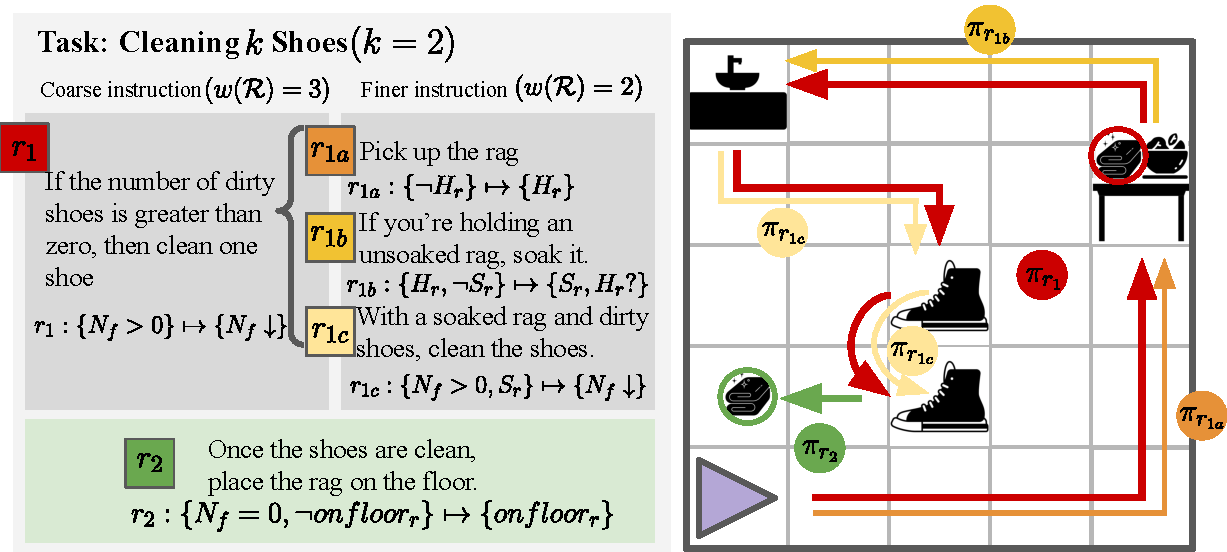
\includegraphics[width=\linewidth]{figures/running_examples.pdf}
    \caption{(Left) Factoring $r_1$ into $r_{1a}$-$r_{1c}$ reduces latent planning complexity via explicit action guidance. (Right) Fine instructions segment the long-horizon coarse trajectory ($\pi_{r_1}$, red).}
    \label{fig:running_example}
\end{figure}

\subsection{Rule Width as a Granularity Measure} % Sec 3.4
\label{subsec:rule_width_granularity}
% (规则宽度作为粒度度量) 核心贡献部分。首先基于宽度理论，定义单条规则的宽度。然后，定义整个指令（即规则集）的宽度为其所有规则宽度的最大值。最后，论证该度量如何对应指令粒度：低宽度=细粒度（提供详细子目标），高宽度=粗粒度（留下更多并发规划需求）。
The width $w(r_i)$ of a rule $r_i$ represents the number of state variables (features) that must be tracked concurrently to fulfill the transition. Formally, for a rule to have width $k$, the agent must coordinate at most $k$ features from $\Phi$ to reach the effect $E_{r_i}$ from a state satisfying $C_{r_i}$ \citep{DBLP:conf/ecai/LipovetzkyG12}.

We define the granularity of an instruction $\mathcal{R}$ by its width-based planning bottleneck: the maximum width among its constituent rules: $w(\mathcal R) = \max_{r_i \in \mathcal R} w(r_i)$.

% (贯穿实例) 使用一个具体任务（例如您提到的“铺设木地板”），完整演示上述过程：任务的目标、定义的特征、为不同粒度设计的规则集，以及计算出的规则宽度。用此例直观说明“宽度”如何作为调节指令粒度的旋钮。

\begin{figure*}[t]
    \centering
    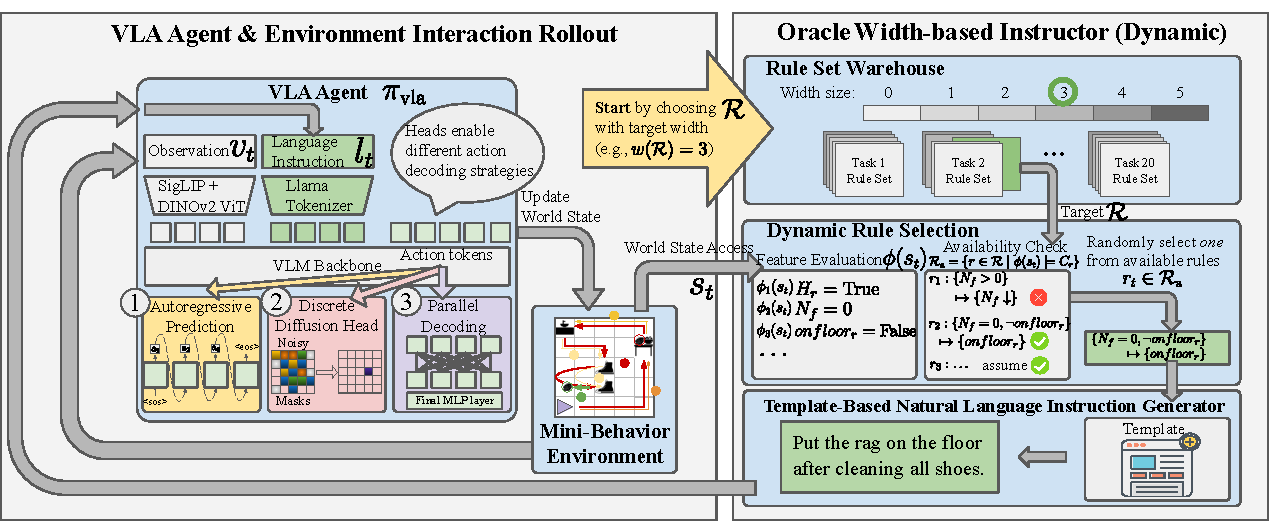
\includegraphics[width=0.85\linewidth]{figures/experiment_illu.pdf}
    \caption{\textsc{Mini-BEHAVIOR-Gran} Experimental Pipeline. We evaluate the impact of instruction granularity across three VLA action-decoding strategies. During inference time, an Oracle Instructor evaluates the current world state to decide available rule set $\mathcal R_a$ and active rule $r_t$. A rule-based natural language instruction $l_t$ is generated accordingly. The process iterates until completion or max steps.}
    \label{fig:experiment_illu}
\end{figure*}



We continue the running example to demonstrate two instruction sets, each representing a different width level, with two variants visualized in \Cref{fig:running_example}. We also append a \textbf{counting feature} in $\Phi$ to track the number of uncleaned shoes, denoted as $N_f$.

\paragraph{Coarse-Grained Instruction ($w(\mathcal R) = 3$ )} This instruction states only the high-level rules and their desired ordering, leaving the internal structure of each sub-task implicit:
\begin{itemize}[leftmargin=*]
    \item $r_1 : \{N_f > 0\} \mapsto \{N_f \downarrow\}$ (clean a shoe; $w=3$)
    \item $r_2 : \{N_f = 0, \neg onfloor_{r}\} \mapsto \{onfloor_{r}\}$ (put the rag on the floor after cleaning shoes; $w=1$)
\end{itemize}

% (Two-column figure spanning the top of the page)Panel A: Admissible Chains. A comparison table of "Working Memory" requirements. Shows how $w=3$ requires a 3-feature tuple, while $w=1$ breaks the task into single-feature "stepping stones."Panel B: Feature Tracking Profile. A plot showing the tuple size (active feature tracking) over the task duration. $w=3$ shows a high, sustained peak; $w=1$ shows a low, consistent baseline.Panel C: The Grounding Gap. A conceptual diagram visualizing the "Informational Void" where the agent must rely on learned biases rather than explicit instructions.

\paragraph{Middle-Grained Instruction ($w(\mathcal R) = 2$ )} This variant decomposes $r_1$ to explicitly state the \emph{soaking} process:
\begin{itemize}[leftmargin=*]
    \item $r_{1a} : \{\neg H_r\} \mapsto \{H_r\}$ (pick up the rag; $w = 1$)
    \item $r_{1b} : \{H_r, \neg S_r \} \mapsto \{S_r, H_r?\}$ (soak the rag)
    \item $r_{1c} : \{N_f > 0, S_r \} \mapsto \{N_f \downarrow\}$ (clean; $w = 2$)
    \item $r_2 : \{N_f = 0, \neg onfloor_{r}\} \mapsto \{onfloor_{r}\}$ (put the rag on the floor; $w = 1$)
\end{itemize}
This rule set is well-formed: it is goal-terminating via $r_2$, and the rules are sequentially reachable, meaning the successor state of any fulfilled rule (that is not the goal) also meets the condition of at least one rule in $\mathcal{R}$. The set is also robust to perturbations: if an agent drops the rag after soaking it ($\neg H_r$), the rule set remains applicable by reverting to $r_{1a}$ to reacquire the rag before proceeding to the cleaning task ($r_{1c}$). 

\noindent \textbf{Width as a Planning Proxy.} Decomposing a task into a rule set $\mathcal{R}$ provides structural scaffolding, guiding the agent through intermediate ``stepping stone'' states. By design, we assume the execution of $r_i$ does not negate established fluents unless explicitly required by $E_{r_i}$. This is the essence of language-guided decomposition. Without this assumption, language guidance would offer no reduction in complexity; the agent would need to track every feature since the initial state.

This intuition is formally grounded in novelty-driven Breadth-First Search \citep{DBLP:conf/aaai/LipovetzkyG17}. By pruning states that fail to achieve a new feature conjunction of size $\le k$, search complexity is bounded by $O(|\Phi|^k)$. Thus, trajectories that unnecessarily negate an already-achieved precondition $C_{r_i}$ (unless required by $E_{r_i}$) are longer than those preserving it and are pruned from the optimal frontier. Consequently, features in $C_{r_i}$ that are already true are effectively treated as invariants, and the active coordination $w$ reduces to the incremental features needed for the next subgoal. For instance, while the monolithic task requires coordinating $\{H_r, p_s, T_s\}$ ($w=3$, \Cref{tab:q3_cross_granularity}), the instruction $r_{1b}$ leverages the fact that $H_r$ is pre-established. By treating $H_r$ as a fixed invariant, the search width $w$ reduces to the novel features $\{p_s, T_s\}$, yielding $w=2$.

% Fine-grained instructions decompose high-width transitions into low-width sequences, displacing computational complexity from internal agent reasoning to explicit textual guidance. This narrows the grounding gap by reducing the latent coordination required to map language to valid action sequences.




% the width $w(r)$ is the smallest $k$ such that IW($k$) solves $r$. Consider $r_{1b}$ (soaking the rag): if the instruction were expressed as a isolated transition $\{\neg S_r\} \mapsto \{S_r\}$, an agent would need to concurrently coordinate three features: holding the rag ($H_r$), reaching the sink ($p_s = 0$), and toggling the tap (sink) ($T_s$). However, because $r_{1b}$'s precondition requires $H_r$ to be established (via $r_{1a}$), and given that IW search explores states in breadth-first order, any plan that undoes an established feature is necessarily longer than one that preserves it and is subsequently pruned as suboptimal. Hence, the agent can treat $H_r$ as a maintained rather than an actively tracked feature. This reduces the concurrent feature tracking to $\langle T_s, p_s = 0 \rangle$, yielding $w(r_{1b})= 2$. Although the VLA agent does not perform explicit IW search, this width serves as a rigorous proxy for the inherent planning burden imposed by the instruction. The higher rule count and denser preconditions is the explicit indicators of finer instruction granularity. This shift displaces the planning complexity to explicit structural textual guidance. The resulting training data exhibits a more direct language-to-action mapping, thereby reducing the grounding gap that VLA agents must learn to bridge.



% \paragraph{Fine-grained Instruction ($w=1$)} This variant further decomposes the task into six rules where each transition addresses at most one feature change. The task is fully serialized into three stages: preparation ($r_1: \{\neg H_r\} \mapsto \{H_r\}$; $r_2: \{\neg T_s\} \mapsto \{T_s\}$; $r_3: \{H_r, T_s, \neg S_r\} \mapsto \{S_r\}$); cleaning ($r_4: \{N_f > 0, \neg H_r, S_r\} \mapsto \{H_r\}$; $r_5: \{N_f > 0, H_r, S_r\} \mapsto \{N_f \downarrow\}$); and storage ($r_6: \{N_f = 0, \neg onfloor_{r}\} \mapsto \{onfloor_{r}\}$). The higher rule count and denser preconditions is the explicit indicators of increased instruction granularity. This shift displaces the planning complexity to explicit structural textual guidance. The resulting training data exhibits a more direct language-to-action mapping, thereby reducing the grounding gap that VLA agents must learn to bridge.

To communicate these rules to language-guided embodied agents, we translate each rule into a natural-language sentence via a template-based generator. These templates verbalize the features within each rule; e.g., $\{\hlA{$H_r$}, \hlB{$\neg S_r$}\} \mapsto \{\hlC{$S_r$}\}$ is realized as ``If you are \hlA{holding the rag} but \hlB{the rag is not yet soaked}, \hlC{soak the rag}.'' This construction preserves the granularity differences defined by the rule width. Additional language prompt examples are provided in \Cref{app_sec:prompt_examples}.


\section{Mini-BEHAVIOR-Gran Benchmark}
\label{sec:benchmark}
% Step 1: 首先介绍我们想要什么的benchmark: 要能够更isolate instruction granularity 的影响，然后visual perception difficulty 和 low level action control complexity 都要简单（从而避免confound）
% 然后我们看一下之前mini behavior 自己是怎么justify自己的：
% We present a new simplified benchmark, Mini-BEHAVIOR, that provides the benefits of simple
% benchmarks for fast prototyping and training, while keeping the most relevant problem structure and
% the characteristics from the task-level decision-making challenge in BEHAVIOR: the long-horizon,
% heterogenousness of the activities, and the multi-object, multi-state, high variability of household
% environments. Mini-BEHAVIOR re-defines BEHAVIOR tasks in a novel 3D Gridworld environment
% with support for procedural generation for potentially infinite variants of each task.

% Step 2: 因此我们选择在mini behavior的基础上进行扩展。然后之说我们在appendix 上有更详细的justification. Details on why these environments are \textbf{preferred over other test benchmarks} are provided in \Cref{app_sec:ant_defense_test_env}.

To disentangle the influence of instruction granularity in agent performance, we seek an environment that (1) retains long-horizon and heterogeneous activities so that instruction guidance meaningfully modulates the planning demand, while (2) simplifies perception and low-level control to avoid confounding factors. As such, we use \textsc{Mini-BEHAVIOR} \citep{jin2023minibehavior} as our testbed. Detailed justification for our choice over other environments is provided in \Cref{app_sec:ant_defense_test_env}.

% Step 3: 要不要给一个表写上是哪些20 tasks 然后我提供的granularity levels for each task 有哪些（我感觉可以放在appendix里）
% Step 4: 介绍offline dataset construction 是用了 BFWS planner 来 generate plans corresponding to the rule sets. 然而在inference time, 我们使用oracle instructor 来 generate filter and select valid rule to generate instruction by accessing the internal state of the environment to get current feature valuations $\phi(s)$ 然后 check which rule conditions are satisfied (需要formula), 然或说 \Cref{fig:experiment_illu} 进行说明。

We introduce \textsc{Mini-BEHAVIOR-Gran}, the first benchmark enabling controlled study of instruction granularity via \emph{rule width}. Over 20 tasks sharing a feature set $\Phi$, we design rule sets at up to six width levels, all verified solvable. During inference, an oracle instructor monitors the current feature vector $\phi(s_t)$, selects an available rule $r_t$ from the task's rule set, and translates it via a template into a natural language instruction $l_t$. This guarantees that performance differences reflect grounding ability alone, not stochastic instruction quality (see \Cref{fig:experiment_illu}). The instruction $l_t$ and current observation $v_t$ are then fed to the learning-based agent to predict action chunks $(a_t, ..., a_{t+k}) \sim \pi_{\text{agent}}(\cdot \mid v_t, l_t)$.


% Step 5: 上价值，need to highlight that our finding can Transfer beyond Mini-BEHAVIOR，我门的feature set 是specific to household domains, 但是不是specific to mini-behavior. 

% \textsc{Mini-BEHAVIOR-Gran} serves as a first-of-its-kind testbed for studying instruction granularity in VLA. By anchoring to an environment-wide feature abstraction $\Phi$, our formalization remains cross-task available, thereby supporting an open-ended set of activities defined over $\Phi$. Moreover, new features can be appended to support additional domains while keeping existing ones intact, allowing extension to other embodied environments that support symbolic state abstraction.

\begin{figure*}[t]
    \centering
    \begin{minipage}[t]{0.30\textwidth}
        \centering
        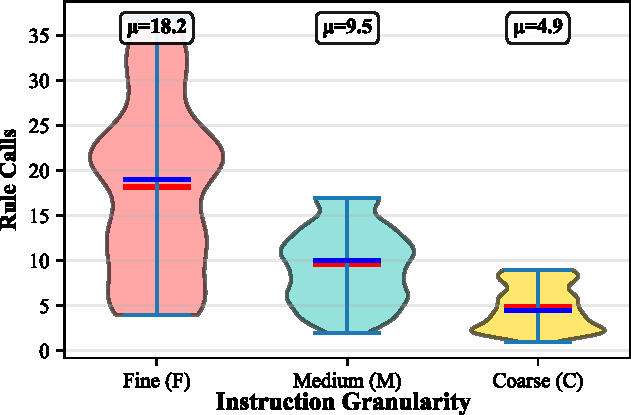
\includegraphics[width=\linewidth]{figures/q1_rule_call_dist.pdf}
        \captionof{figure}{Rule call distribution across instruction granularities. \# of rule calls decreases with coarser instructions. It decouples instruction length from width.}
        \label{fig:q1_rule_call_dist}
    \end{minipage}
    \hfill
    \begin{minipage}[t]{0.30\textwidth}
        \centering
        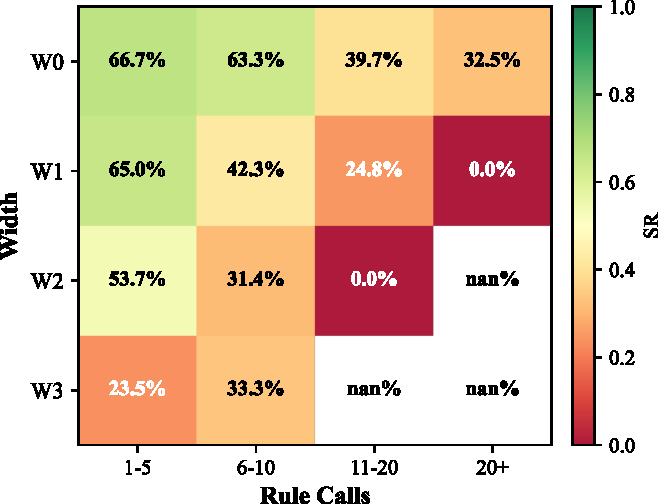
\includegraphics[width=\linewidth]{figures/q1_width_vs_task_horizon_heatmap.pdf}
        \captionof{figure}{Impact of width and horizon on SR. SR decays with task horizon; larger instruction width imposes an additional burden even when horizon is fixed.}
        \label{fig:q1_width_vs_task_horizon_heatmap}
    \end{minipage}\hfill
    \begin{minipage}[t]{0.33\textwidth}
        \centering
        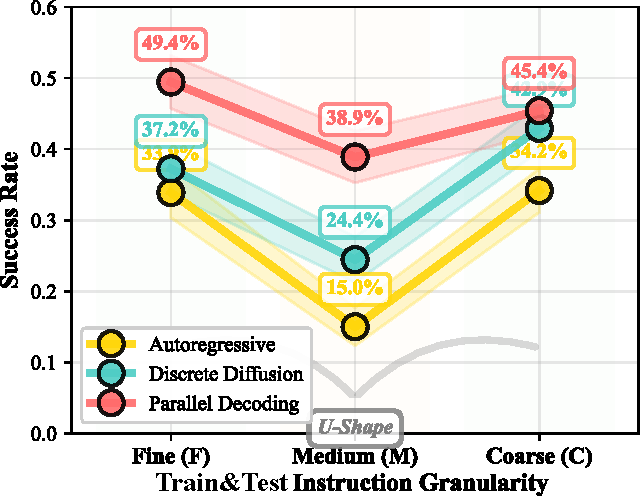
\includegraphics[width=0.9\linewidth]{figures/q1_main.pdf}
        \captionof{figure}{In-Distribution (matched train/test) SR across granularities (i.e., train Fine $\rightarrow$ test Fine, etc). A non-monotonic U-shaped trend appears.}
        \label{fig:q1_learning_curves}
    \end{minipage}
\end{figure*}

\section{Experiments}
\label{sec:experiments}
% **话术：** “由于这是首个系统性研究指令粒度的 Benchmark，我们的实验重点在于揭示 **Instruction Granularity ($w$)** 与 **Learning Burden** 之间的本质联系。我们不追求在多个异构 Benchmark 上刷榜，而是在一个受控的环境中探索指令粒度对 VLA 的影响函数。”
\subsection{Experimental Setup}
\paragraph{Task Suite \& Training.} We use \textsc{Mini-BEHAVIOR-Gran}, which contains 20 complex tasks sharing the same feature set $\Phi$. We further classify instruction granularity into three \emph{relative} classes of \emph{Fine (F)}, \emph{Medium (M)}, and \emph{Coarse (C)} via per-task quantile binning. In most cases, this mapping corresponds to $w=0$ for Fine, $w=1$ for Medium, and $w \ge 2$ for Coarse. We evaluate seven training settings: (1) \textbf{Pure F/M/C} ($1\!:\!0\!:\!0$): trains exclusively on one granularity class; (2) \textbf{Centroid} ($1\!:\!1\!:\!1$): uniformly sample from all three classes; (3) \textbf{Axial F/M/C} ($3\!:\!1\!:\!1$): emphasizes one class with some exposure to the other classes. Our dataset provides 50 training and 10 evaluation instances per task, each paired with reference trajectories generated by \textsc{BFWS} width-based planner from \citet{DBLP:conf/aaai/LipovetzkyG17} (see \Cref{app_sec:minibehavior_gran_details} for details).

% \paragraph{Relative Instruction Binning.} A significant challenge in evaluating instruction granularity is that different tasks possess inherently different structural depths; for instance, opening_packages may only support a maximum width of $w=1$, whereas cleaning_the_kitchen extends to $w=5$. To maintain a balanced evaluation across this heterogeneous suite, we implement a per-task quantile-based binning strategy. For each domain, we sort the available symbolic widths and partition them into three relative levels: Fine (Low), Medium, and Coarse (High). In cases with limited width availability, we apply a priority-fill heuristic to ensure every task contributes to all three experimental categories. This normalization allows us to observe universal performance trends across the complexity spectrum, independent of the absolute planning width of any specific task.



\paragraph{Action-Decoding Archetypes.} The primary architectural difference among latest VLA models lies in their action-decoding strategies \citep{zhong2025survey}. Hence, we employ a unified VLM backbone but vary three representative action-decoding strategies (see \Cref{fig:experiment_illu} left panel): (1) \textbf{Autoregressive} (AR), exampled by RT-2 \citep{DBLP:conf/corl/ZitkovichYXXXXW23}, OpenVLA \citep{DBLP:conf/corl/KimPKXB0RFSVKBT24} and others \citep{DBLP:journals/tmlr/ReedZPCNBGSKSEBREHCHVBF22,DBLP:conf/icml/HuangYMLLW0ZJ024,DBLP:conf/icra/ONeillRMGPLPGMJ24} that predict actions sequentially via causal attention; (2) \textbf{(Discrete) Diffusion}, which uses diffusion process for action chunk prediction \citep{pmlr-v305-black25a,bjorck2025gr00t,shukor2025smolvla}. We employ discrete diffusion \citep{liang2025discrete} for compatibility with the discrete action space of our testbed; (3) \textbf{Parallel Decoding}, utilizing bidirectional attention for single-pass action prediction to improve throughput, as demonstrated by OpenVLA-OFT \citep{kim2025fine}, PD-VLA \citep{DBLP:conf/iros/SongCDZZZGLWWML25} and other variants \citep{yin2025deepthinkvla,wang2025bitvla,xiao2025ava}. Details on model hyperparameters, hardware and training schedules are in \Cref{app_sec:implementation_details}.

\subsection{Establishing the Yardstick: Decoupling Horizon from Width}
\label{sec:decoupling}



A critical confounder in evaluating language grounding complexity is the task sequence length. However, in language-guided execution, instructions inherently decompose long-horizon tasks into segments. Consequently, the relevant measure of sequential burden shifts from the raw atomic horizon (total action steps) to the instruction horizon, i.e., the number of rule calls issued by the instructor.

To isolate rule width from sequential burden, we train a single agent across all tasks using the Centroid configuration, ensuring balanced exposure across all granularity levels. This approach holds the distribution of atomic horizons constant, allowing us to isolate how instruction granularity and the frequency of rule calls affect performance. \Cref{fig:q1_rule_call_dist} shows that fine-grained instructions ($w=0$) decompose the task into numerous low-width rule calls; coarse instructions ($w \ge 2$), by contrast, yield fewer rule calls.
\begin{figure*}[t]
    \centering
    \begin{minipage}[t]{0.56\textwidth}
        \centering
        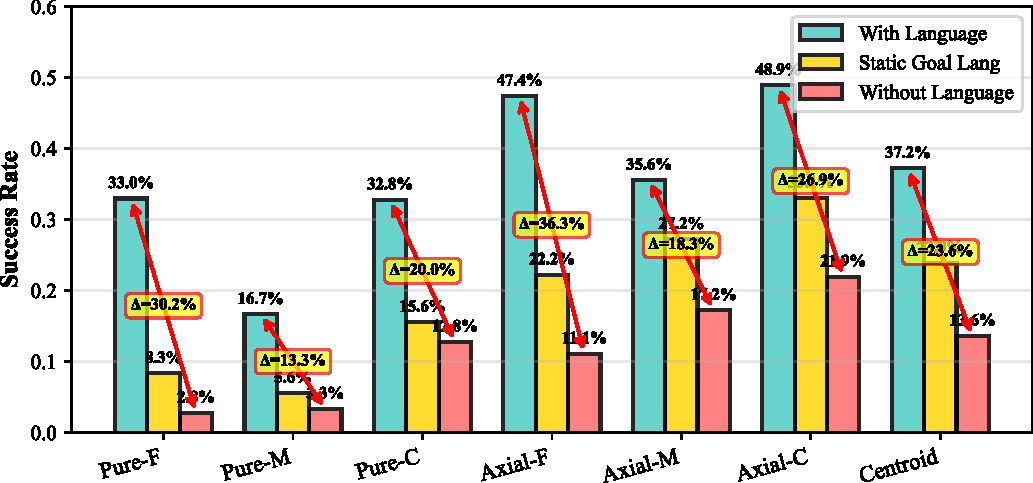
\includegraphics[width=\linewidth]{figures/q5_sr_diff_by_training_setup.pdf}
        \captionof{figure}{Smaller SR gaps indicate a shift towards shallow grounding. Under semantic perturbation, the Pure-C setting exhibits tiny variance ($2.8\%$) between \textit{w/ goal lang} and \textit{w/o lang}.}
        \label{fig:sr_diff_by_training_setup}
    \end{minipage}\hfill
    \begin{minipage}[t]{0.40\textwidth}
      \centering
    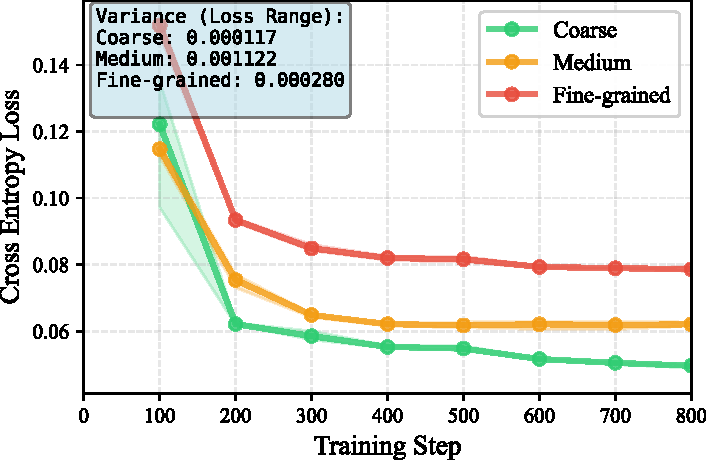
\includegraphics[width=\linewidth]{figures/q7_loss_comparison.pdf}
    \captionof{figure}{VLM instruction-prediction Cross Entropy (CE) loss across granularities and 3 seeds. Larger CE loss indicates lower $P(l \mid v)$.}
    \label{fig:cross_entropy_loss_comparison}
    \end{minipage}
\end{figure*}

\begin{figure}[t]
    \centering
    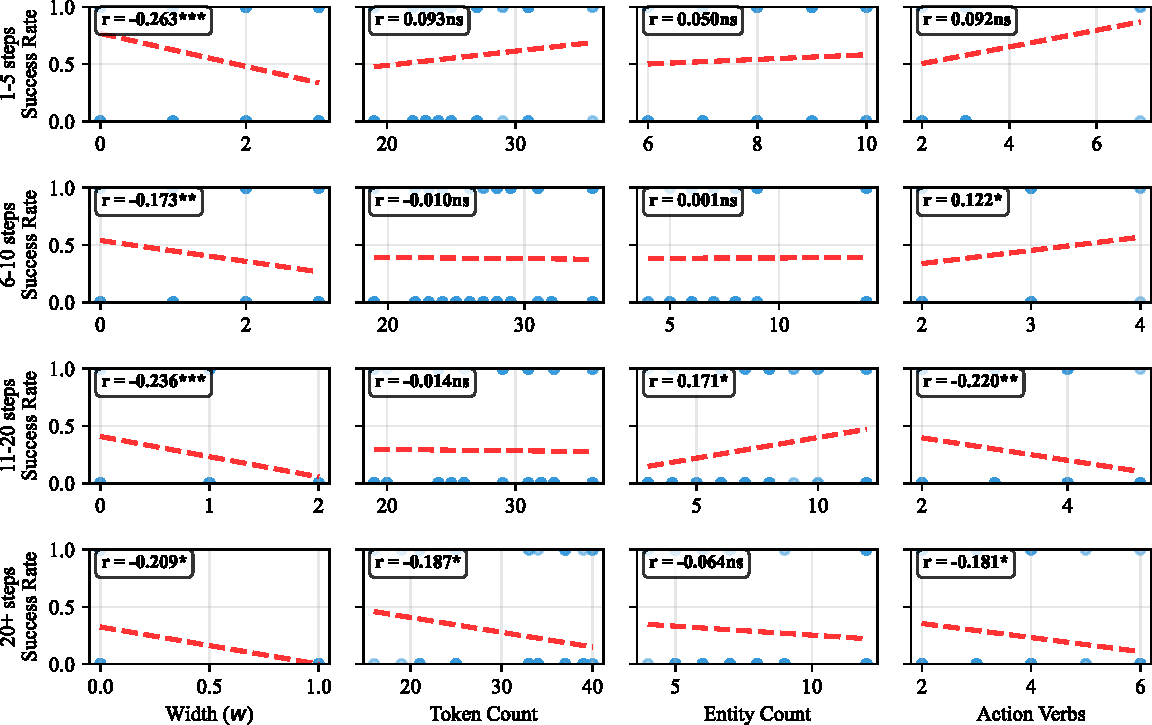
\includegraphics[width=\linewidth]{figures/q8_scatter_by_horizon.pdf}
    \caption{Metric-success correlation by task-horizon.}
    \label{fig:q8_scatter_by_horizon}
\end{figure}


To assess whether $w$ serves as an effective indicator of latent planning demand for learning-based agents, we analyze \Cref{fig:q1_width_vs_task_horizon_heatmap}. The heatmap reveals a strict monotonic decay in Success Rate (SR) as rule width increases. Also, for a fixed $w$, SR decays as rule calls increase, mirroring greater sequential horizon complexity. This confirms $w$ as a horizon-independent measure of the intrinsic planning demand imposed by instruction granularity.

\paragraph{Width vs. Syntactic Heuristics.} 
We evaluate whether $w$ captures language grounding complexity better than common linguistic heuristics: token count, entity count, and action verbs. \Cref{fig:q8_scatter_by_horizon} shows $w$ is the only metric that exhibits a statistically significant and consistently \emph{negative} correlation with SR across task horizons. Action Verbs correlate significantly but flip direction across horizons, while Token Count turns negative only in the longest bin (20$+$ steps). These heuristics are inconsistent compared to $w$ (see details in \Cref{app_sec:additional_experimental_results}).


\subsection{The U-Shaped Paradox and Capacity Cap}

To establish a baseline, we train models using the \emph{Pure F/M/C} setting. the models are trained and evaluated on the same granularity class. As shown in \Cref{fig:q1_learning_curves}, all VLA archetypes exhibit a non-monotonic \emph{U-shaped performance curve}. 

At the fine extreme ($w=0$), where instructions require minimal latent reasoning to be grounded into actions, models achieve high performance. Performance then decreases at medium granularity ($w=1$), before unexpectedly rebounding at the coarse regime ($w \ge 2$). This contradicts the assumption that higher planning width should monotonically degrade learning.

\subsection{Mechanistic Probe: The Grounding Valley}
Why does performance rebound at $w \ge 2$? We show this arises from increasing \emph{instruction predictability} $P(l|v)$, which enables agents to bypass language and exploit visual-dominant policy.

Following prior work \citep{fei2025liberoplus}, we use $\Delta\mathrm{SR}_{\text{w/ - w/o}}$ as a basic measure of language grounding. To further isolate grounding effects, we conduct another intervention: replacing full instructions with high-level static goal descriptions (\Cref{fig:sr_diff_by_training_setup}). When language is entirely removed, fine-trained policies suffer a severe $36.3\%$ drop, whereas coarse-trained policies show a smaller $20.0\%$ gap. Also note that under reduced informativeness (\textit{w/ goal lang}), the Pure-C policy exhibits a negligible $2.8\%$ advantage over having no language at all ($15.6\%$ vs. $12.8\%$). This indicates that policies trained on coarse instructions develop a shallow grounding behavior: language is not deeply integrated into their decision-making. Consequently, when instructions are reduced to generic goals, their performance barely differs from the vision-only baseline.

\begin{figure*}[t]
    \centering
    \noindent
    \begin{minipage}[b]{0.60\textwidth}
        \centering
        \small
        \resizebox{\textwidth}{!}{%
        \begin{tabular}{lccccc}
        \toprule
        \textbf{Training Setup} & \textbf{Width 0} & \textbf{Width 1} & \textbf{Width 2} & \textbf{Width 3} & \textbf{Width $\ge 4$} \\ 
        \midrule
        Pure-F          & 34.9\% & 16.9\% & 10.8\% & 1.0\%  & 0.0\% \\
        Pure-M          & 12.2\% & 22.0\% & 11.7\% & 0.0\%  & 0.0\% \\
        Pure-C          & 26.3\% & 33.3\% & 32.9\% & 22.9\% & 0.0\% \\ 
        \midrule
        Axial-F         & 50.2\% & 53.3\% & 48.8\% & 34.3\% & 0.0\% \\
        Axial-M         & 44.7\% & 43.5\% & 45.8\% & 29.5\% & 0.0\% \\
        Axial-C         & \textbf{55.7\%} & 52.2\% & 50.8\% & \textbf{37.1\%} & 0.0\% \\ 
        \midrule
        Centroid (Mix)  & 42.7\% & 38.4\% & 40.8\% & 28.6\% & 0.0\% \\
        \bottomrule
        \end{tabular}%
        }
        \captionof{table}{The x-axis are test instruction width, y-axis are training setup. Transfer is asymmetric: train coarse $\rightarrow$ test fine works, but train fine $\rightarrow$ test coarse does not. Mixed-granularity improves overall.}
        \label{tab:q3_cross_granularity}
    \end{minipage}\hfill
    \begin{minipage}[b]{0.35\textwidth}
        \centering
        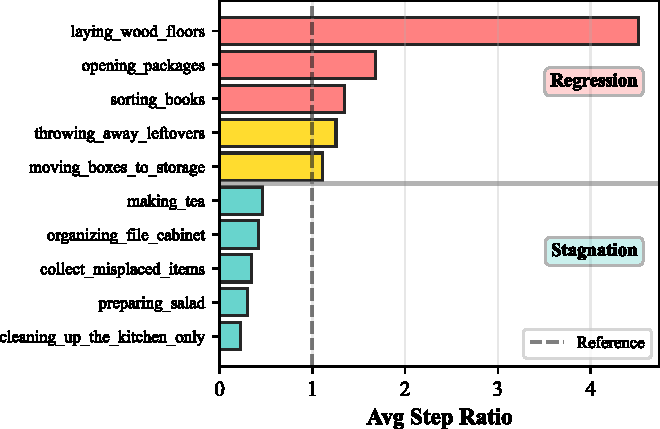
\includegraphics[width=\linewidth, keepaspectratio]{figures/q4_failure_type_extreme_task_example.pdf}
        \captionof{figure}{Low-width but long task horizon (e.g., laying woods) tends to cause regression, while high-width stagnates.}
        \label{fig:q4_failure_modes}
    \end{minipage}
\end{figure*}


\paragraph{The Predictability Driver: Why Reliance Shifts.}
We hypothesize that this behavioral shift originates from coarse instructions being statistically more predictable from vision. Formally, consider a surjective mapping $f$ from fine-grained labels $L_{\text{fine}}$ to coarser ones $L_{\text{coarse}}$. The conditional probability of a coarse label aggregates its fine-grained constituents: $P(c_j | v) = \sum_{l_i \in f^{-1}(c_j)} P(l_i | v)$. The increasing predictability of coarse instructions reduces the marginal information contributed by language, making it easier for agents to minimize task loss by relying primarily on visual observations, thereby favoring the development of visuo-motor shortcuts over costly cross-modal alignment. We confirm this predictability empirically by training a VLM (Qwen3-VL-4B via LoRA) to act as an trained instructor, predicting instructions from visual observations. As \Cref{fig:cross_entropy_loss_comparison} shows, Cross-Entropy (CE) loss decreases monotonically with coarseness (Fine: 0.078, Medium: 0.063, Coarse: 0.047), a relative drop of $40\%$ from Fine to Coarse. Together, these results form a complementary chain: probability aggregation explains \emph{why} $P(l|v)$ increases, CE loss empirically confirms the increase, and the perturbation $\Delta$SR quantifies the resulting visuo-motor shift.

Thus, we attribute this U-shaped behavior to how the agent dynamically shifts its reliance on text versus vision across different rule widths:



\begin{itemize}[leftmargin=*]
    \item \textbf{Fine ($w=0$):} \emph{Deep Grounding.} Low $P(l|v)$ (high CE loss, \Cref{fig:cross_entropy_loss_comparison}) means language provides unique information. Combined with low-width grounding burden (\Cref{sec:decoupling}), the model reliably maps instructions to actions, yielding high SR (\Cref{fig:q1_learning_curves}).

    \item \textbf{Medium ($w=1$):} \emph{The Alignment Trap.} At this width, grounding complexity increases while $P(l|v)$ remains moderate: not yet high enough to exploit reliable visuo-motor shortcuts. The model must attempt language grounding but struggles with its inherent difficulty. This intermediate regime, caught between hard alignment and insufficient shortcuts, yields the lowest performance.

    % 修改点 4：Tone down Modality Collapse
    \item \textbf{Coarse ($2 \le w \le 3$):} \emph{Reduced Language Reliance.} High $P(l|v)$ incentivizes a visual-dominant policy: aligning vision to action is easier than learning cross-modal grounding. This yields high in-distribution scores but at the cost of language grounding capability.

    \item \textbf{Capacity Cap ($w \ge 4$):} \emph{Cognitive Overload.} Mirroring the $O(|\Phi|^4)$ complexity barrier of symbolic planners \citep{DBLP:conf/aaai/LipovetzkyG17}, VLA agents performance uniformly collapses at $w \ge 4$ (\Cref{tab:q3_cross_granularity}). This convergence suggests $w$ as a fundamental representational bottleneck shared by both symbolic and neural paradigms.
\end{itemize}

% 修改点 5：加入 11.1% vs 2.8% 的绝杀对比，证明你的方法有效
\paragraph{Deepening Grounding via Axial Training.} 
Having diagnosed this shallow reliance as a byproduct of high predictability, we hypothesize that increasing the diversity of the training language space $L$ should artificially lower the average $P(l | v)$, forcing the agent to structurally re-engage with the text. Our mixed-granularity training confirms this mechanism. All mixed-granularity models exhibit substantially larger $\Delta\mathrm{SR}$ gaps compared to their \emph{Pure-X} counterparts. Among these, the fine-weighted mixture \emph{Axial-F} emerges as the optimal structural compromise: it achieves an overall success rate, while maintaining a significantly larger $\Delta\mathrm{SR}$.



\subsection{Other Results}
\paragraph{Asymmetric Generalization.} We observe an asymmetric transfer pattern (\Cref{tab:q3_cross_granularity}): coarse-trained models successfully zero-shot transfer to fine-grained instructions, but fine-trained models fail on coarse-grained ones. This asymmetry aligns with our $\Delta\mathrm{SR}$ analysis: coarse training induces a visual-dominant policy, hence perturbing or refining the instruction yields minimal behavioral change. Conversely, fine training induces tight coupling with language, making the policy brittle when detailed guidance is withdrawn.


\paragraph{Failure Modes.} Agent failure distributions bifurcate strictly with width (\Cref{fig:q4_failure_modes}). Low-width, long-horizon tasks predominantly suffer from \emph{regression}: the agent violates previously satisfied fluents and cycles back to prior states, reflecting subgoal serialization failures. High-width tasks ($w \ge 3$), by contrast, exhibit \emph{stagnation}: the agent freezes, unable to resolve concurrent feature dependencies ($O(|\Phi|^w)$) required to initiate a valid state transition. This dichotomy mirrors the width-based complexity landscape (see \Cref{app_sec:additional_experimental_results} for details).


\section{Conclusion}
\label{sec:conclusion}
% 在论文的局限性部分，主动、诚恳地讨论上述部分问题（如环境的简化、动态指导的理想化），并阐述未来如何在本工作基础上进行扩展研究（如在更复杂环境中验证、研究稀疏指令下的规划）。这能展现您思考的全面性，并化解审稿人的部分质疑。


This work introduces rule width ($w$) as a cross-task formalism for instruction granularity and demonstrates that it correlates with language grounding difficulty in learning-based agents. We observed a non-monotonic relationship between granularity and performance, driven by a trade-off between instruction predictability ($P(l | v)$) and latent planning complexity. We demonstrate that mixed-granularity training balances language sensitivity without sacrificing the robust visual reasoning skills learned from coarse trajectories.


\section{Limitations}
\label{sec:limitations}

\paragraph{Discrete Action Spaces.} We evaluate our framework in environments with discrete action spaces, a common abstraction in language-conditioned embodied AI (e.g., ALFWorld-based agent \citep{xiong-etal-2025-mpo, kim-etal-2025-reflact}) and LLM-based agent systems \citep{DBLP:conf/iclr/QinLYZYLLCTQZHT24, DBLP:conf/nips/PatilZ0G24}, where high-level reasoning is decoupled from low-level execution via skill primitives or API calls. This choice is intentional: it isolates symbolic planning from continuous control noise, allowing us to cleanly attribute observed effects to instruction granularity. However, extending this granularity-aware framework to hybrid discrete-continuous or continuous action spaces remains essential for real-world robotics applications, where low-level motor commands interact with high-level linguistic abstractions.

\paragraph{On the Oracle Instructor Setup.} A potential concern is that providing the active rule via an Oracle simplifies the task to single-step grounding. However, we argue that the \textbf{latent planning demand} $w$ is an intrinsic property of the instruction-to-action mapping. Even when the ``what to do'' is provided, the agent must still coordinate $w$ concurrent features to achieve the transition. Our findings that performance collapses at $w \ge 4$ \emph{despite} Oracle guidance (\Cref{tab:q3_cross_granularity}) demonstrates that the grounding gap is a fundamental bottleneck in the learning process.

% \paragraph{Grid-Based Environment.} We acknowledge that our experiments are conducted in a 2D grid-world environment with simplified visual dynamics. This raises legitimate questions about external validity. However, we argue that this simplification actually provides a lower bound on the grounding difficulty: if VLA models struggle to maintain concurrent feature dependencies even in visually simple environments, this challenge will likely be exacerbated in photorealistic 3D settings with complex occlusions, lighting variations, and rich textures. Recent evidence supports this view: state-of-the-art VLMs achieve only 23-27\% SR in photorealistic 3D exploration tasks \citep{pardyl2025flysearch}, and exhibit particular difficulty with non-photorealistic inputs such as cartoons and line art \citep{kim2025make}. Our findings thus highlight a fundamental challenge in language grounding that is not merely a byproduct of visual complexity.



% Bibliography entries for the entire Anthology, followed by custom entries
%\bibliography{anthology,custom}
% Custom bibliography entries only
\bibliography{custom}

\appendix
% Start of appendices customization

\section{Technical Appendix}

\section*{Appendix Table of Contents}
\begin{enumerate}[leftmargin=*]
    \item \textbf{Anticipatory defense on the choice of test environments and metrics} (\Cref{app_sec:ant_defense_test_env}) \\
    Justification for using \textsc{Mini-BEHAVIOR} over alternatives (e.g., iGibson, CALVIN) based on controllability, symbolic abstraction, and isolation of language-grounding challenges.
    \item \textbf{Symbolic Representation of the Embodied Task} (\Cref{app_sec:classical_prob_def})
    Formal definition of states, actions, and planning problems using classical STRIPS/PDDL semantics.
    \item \textbf{Details of the \textsc{Mini-BEHAVIOR} Environment} (\Cref{app_sec:minibehavior_details})
    Overview of scene layout, object types, action space, and perception model.
    \item \textbf{Details of the \textsc{Mini-BEHAVIOR-Gran} Extension} (\Cref{app_sec:minibehavior_gran_details})
    Procedure for generating multi-granularity instructions, details on the feature set, oracle instructor, and dataset construction.
    \item \textbf{Rule Set and Natural Language Prompt Examples} (\Cref{app_sec:prompt_examples})
    Details of the rule set bank of 20 tasks and sample generated instructions at different granularities.
    \item \textbf{Implementation Details} (\Cref{app_sec:implementation_details})
    Model architecture (Prismatic-7B backbone, SigLIP+DINOv2 visual encoders), training hyperparameters, optimizer settings. VLM Predictor architecture and training details.
    \item \textbf{Additional Experimental Results} (\Cref{app_sec:additional_experimental_results})
    Extended analysis and ablations.
\end{enumerate}

\section{Anticipatory defense on the choice of test environments and metrics}
\label{app_sec:ant_defense_test_env}

% 主动承认并界定研究范围：明确指出，本工作的首要目标是机理研究，而非追求极致的现实仿真。Mini-BEHAVIOR在保留家庭任务的长视距、多对象、状态依赖等高层级决策复杂性的同时，主动剥离了低层级感知与控制的噪音。这使我们能够将模型失败更清晰地归因于语言grounding和规划问题，而非纹理识别或连续运动控制。

% 使用“先理解，再扩展”的研究范式论证：引用经典研究范式——先在受控的简化环境中理解核心机理，再将验证过的假设推广到更复杂的场景。可以说明，我们的形式化方法（规则宽度）是任务和平台无关的，未来可以在更复杂的仿真器中复用同一套指令生成与控制框架。

% 对比优势：简要对比指出，在iGibson等高级仿真器中，难以程序化地生成海量、精确对应不同规则宽度的指令-轨迹对，且渲染和物理计算成本过高，不利于进行需要大量实验迭代的消融研究。

In this work, we selected Mini-BEHAVIOR as our testbed. This choice is motivated by several key considerations aligned with our research objectives. Our research objective is not to solve the full stack of robotic embodiment (which includes perception, continuous control, and physics), but specifically to isolate and analyze the impact of instruction granularity on language grounding and long-horizon planning.

Therefore, high-fidelity simulators (e.g., iGibson \citep{li2022igibson}, BEHAVIOR-1K \citep{DBLP:conf/corl/0002ZWGSMWLLSAH22}) introduce significant noise through complex texture rendering and continuous motor control. While realistic, these factors act as confounders. When an agent fails in such environments, it is often difficult to attribute the failure to a lack of linguistic understanding (granularity issues) or a failure in low-level execution (e.g., grasping physics or occlusion). Mini-BEHAVIOR retains the high-level decision complexity of household tasks—long horizons, multi-object interactions, and state dependencies—while abstracting away low-level sensorimotor noise.

In the perspective of fast prototyping and iterative experimentation, we have to also consider the rendering and physics simulation costs. Mini-BEHAVIOR's grid-based discrete control and simplified visual representation allow for rapid data generation and model training. 

Another consideration is the diversity of the task structures so that we can systematically vary instruction granularity across a wide range of scenarios. As such, Crafter \citep{hafner2021crafter}, which focuses on survival in a single domain, lacks the diverse task structures needed to obtain robust insights about instruction granularity. 

Table \ref{tab:env_comparison} provides a detailed comparison of Mini-BEHAVIOR against other prominent benchmarks, highlighting why they were less suitable for this specific investigation.

\begin{table*}[t]
\small
\centering
\caption{Comparison of Embodied AI Environments regarding their suitability for studying Instruction Granularity.}
\label{tab:env_comparison}
\begin{tabular}{@{}l>{\raggedright\arraybackslash}p{1.4cm}c>{\raggedright\arraybackslash}p{1.5cm}>{\raggedright\arraybackslash}p{1.7cm}>{\raggedright\arraybackslash}p{4.9cm}@{}}
\toprule
\textbf{Environment} & \textbf{Control} & \textbf{Horizon} & \textbf{Visuals} & \textbf{Symbolic Abstraction} & \textbf{Limitation} \\
\midrule
\textbf{Mini-BEHAVIOR}(*) & Discrete & Long & Grid & \textbf{Support} & \textbf{Ideal balance:} Supports symbolic state abstraction; diverse task suite; removes control noise while retaining logic complexity. \\
\textbf{Crafter} & Discrete & Long & Cartoon & Partial & Single task suite (survival); partially observable (memory heavy); few object types. \\
\textbf{Meta-World} & Continuous & Short & 3D & No & Continuous control; no symbolic abstraction; focus on multi-task RL/manipulation, not long-horizon planning. \\
\textbf{LIBERO} & Continuous & Short & 3D & No & Robotic arm focus; continuous control; no symbolic abstraction; VLA success rate already saturated (tasks relatively easy). \\
\textbf{RoboTwin 2.0} & Continuous & Short & 3D & No & Continuous control; no symbolic abstraction; dual-arm manipulation focus; hard to segment expert trajectories and construct granular instructions. \\
\textbf{CALVIN} & Continuous & Medium & 3D & No & Hard to design instruction granularity due to continuous action space (though provides diverse language); confounds planning with control difficulties. \\
\textbf{ALFRED} & Discrete & Long & 3D Photo & Support & 3D partially observable; poor infrastructure support for VLA training; high rendering cost. \\
\textbf{iGibson / BEHAVIOR-1K} & Continuous & Long & 3D Photo & Partial & Good for long-horizon tasks, but 3D realistic vision context becomes a confounder. \\
\bottomrule
\end{tabular}%
\end{table*}

\section{Symbolic Representation of the Embodied Task}
\label{app_sec:classical_prob_def}


We formalize the Mini-BEHAVIOR environment as a deterministic grid-based symbolic world. This allows us to represent the challenge as a classical planning problem $\mathcal{P} = \langle \mathcal{F}, \mathcal{A}, s_0, G \rangle$, where:
\begin{itemize}[leftmargin=*]
    \item $\mathcal{F}$ is a finite set of propositional fluents representing the state variables of the environment (e.g., object locations, states like \textit{cooked} or \textit{open}).
    \item $\mathcal{A}$ is a finite set of actions available to the agent.
    \item $s_0 \subseteq \mathcal{F}$ is the initial state configuration.
    \item $G \subseteq \mathcal{F}$ is the goal condition that must be satisfied.
\end{itemize}
A state $s \in \mathcal{S}$ is defined as a truth valuation over $\mathcal{F}$, with the state space $\mathcal{S} \subseteq 2^\mathcal{F}$ encompassing all valid combinations of fluent truth values.

\section{Details of \textsc{Mini-BEHAVIOR} Environment}
\label{app_sec:minibehavior_details}

To operationalize our formalism, we developed a \textbf{Universal PDDL Domain Model} (available at \url{minibehavior_gran_domain_model.pddl} in the codebase) capable of supporting all 20 household tasks without modification. This unified model comprises over 1,000 lines of PDDL 2.1 definitions and is fully compatible with the LAMA planner. We highly recommend checking the codebase for the complete domain model.

\paragraph{Search Space Characteristics}
\begin{table}[H]
    \centering
    \small
    \caption{Planning complexity in typical tasks.}
    \label{tab:planning_complexity}
    \begin{tabular}{@{}lc@{}}
        \toprule
        \textbf{Metric} & \textbf{Typical Range} \\
        \midrule
        Objects & 15--40 \\
        Grid Locations & 20--60 \\
        Ground Actions & $10^3$--$10^5$ \\
        Plan Length & 50--200 primitive actions \\
        Planning Time (LAMA) & 0.5--300+ seconds \\
        \bottomrule
    \end{tabular}
\end{table}

\section{Details of \textsc{Mini-BEHAVIOR-Gran} Extension}
\label{app_sec:minibehavior_gran_details}

\textsc{Mini-BEHAVIOR} provides the foundational task skeletons, which we extend in \textsc{Mini-BEHAVIOR-Gran} to support multi-granularity instruction generation. A core component of this extension is the definition of a symbolic feature set used to generate rule-based policy sketches.


\subsection{Feature Categories}

The environment defines two primary categories of features: Boolean State Features and Quantitative Features.

\subsubsection{Boolean State Features}
These features evaluate whether a specific object instance satisfies a predicate. They require grounding (binding to specific object instances, e.g., \texttt{rag-01}).

\begin{table}[t]
\centering
\caption{Boolean State Features}
\label{tab:bool_features}
\resizebox{\columnwidth}{!}{%
\begin{tabular}{l|l|l}
\hline
\textbf{Feature} & \textbf{Applicable Objects} & \textbf{Semantics} \\ \hline
\texttt{Holding} & All Items & Is the agent holding the specified object? \\
\texttt{isOpened} & Cabinets, Drawers, Doors & Is the container/door open? \\
\texttt{isToggled} & Sinks, Stoves, Switches & Is the appliance turned on? \\
\texttt{isSoaked} & Rags, Sponges & Is the cleaning tool wet? \\
\texttt{isCleaned} & Shoes, Dishes, Floor & Is the object free of stains? \\
\texttt{isDustFree} & Furniture, Surfaces & Is the object free of dust? \\ \hline
\end{tabular}%
}
\end{table}

\subsubsection{Quantitative and Spatial Features}
These features capture distances, counts, and spatial relationships. Crucially, they support temporal comparison allowing conditions such as ``distance decreased'' or ``count dropped to zero.''

\begin{itemize}[leftmargin=*]
\item \textbf{\texttt{DistanceToNearest(type, condition)}}: Measures the Manhattan distance from the agent to the nearest object of a specific type.
\begin{itemize}[leftmargin=*]
\item \textit{Conditions:} \texttt{=0} (adjacent), \texttt{>0}, \texttt{increase}, \texttt{decrease}, \texttt{change}.
\end{itemize}
\item \textbf{\texttt{Count(type, condition, function)}}: Counts the number of objects of a specific type that satisfy a filter function.
\begin{itemize}
\item \textit{Conditions:} \texttt{=0}, \texttt{>0}, \texttt{increase}, \texttt{decrease}.
\end{itemize}
\end{itemize}

\subsection{Count Functions}
A diverse set of counting functions is implemented to support complex logical conditions (e.g., ``all shoes are clean'' is equivalent to \emph{count\_not\_cleaned == 0}).

\begin{table}[t]
\centering
\caption{Available Count Functions for Rule Definitions}
\label{tab:count_funcs}
\resizebox{\columnwidth}{!}{%
\begin{tabular}{l|l}
\hline
\textbf{Category} & \textbf{Function Description} \\ \hline
\textbf{State-Based} & \texttt{count\_not\_cleaned}: Objects that are currently stained. \\
& \texttt{count\_not\_soaked}: Cleaning tools that are dry. \\
& \texttt{count\_not\_toggled}: Appliances that are turned off. \\
& \texttt{count\_closed}: Containers/doors that are closed. \\
& \texttt{count\_not\_sliced}: Food items that require slicing. \\ \hline
\textbf{Spatial} & \texttt{count\_not\_onfloor}: Objects not placed on the floor layer. \\
& \texttt{count\_isolated}: Objects with no neighbors of the same type. \\
& \texttt{count\_not\_inside\_target}: Objects not contained within a specific furniture. \\
& \texttt{count\_not\_ontop}: Objects not placed on top of a specific surface. \\
& \texttt{count\_not\_near\_target}: Objects not within 1 step of a target type. \\ \hline
\textbf{Task-Specific} & \texttt{count\_incomplete\_salad}: Plates lacking necessary ingredients. \\
& \texttt{count\_not\_complete\_tables}: Tables lacking specific setups (e.g., candles). \\ \hline
\end{tabular}%
}
\end{table}

% \subsection{Activation and Verification Mechanism of Oracle Instructor}
% To support relative conditions (e.g., \textit{``distance decreased''}), features utilize a two-step verification process:
% \begin{enumerate}
% \item \textbf{Precondition Activation:} The feature state is recorded before an action sequence.
% \item \textbf{Effect Verification:} The feature is checked after execution against the stored value.
% \end{enumerate}
% This mechanism is essential for defining granular instructions that describe \textit{progress} (e.g., ``move closer to the sink'') rather than just static states.


\subsection{Reference Plan Generation and Task Complexity Analysis} \label{app_sec:ref_plan_gen}

While the original \textsc{Mini-BEHAVIOR} framework provides the high-level skeletons for household activities, it does not provide reference plans by default. Thus, we utilize the \textsc{BFWS} (Best-First Width Search) classical planner to generate reference plans for all 20 tasks in \textsc{Mini-BEHAVIOR-Gran}. These reference plans serve as the ground truth for our agents and allow us to quantitatively categorize the complexity of each task.

\begin{figure*}[t]
    \centering
    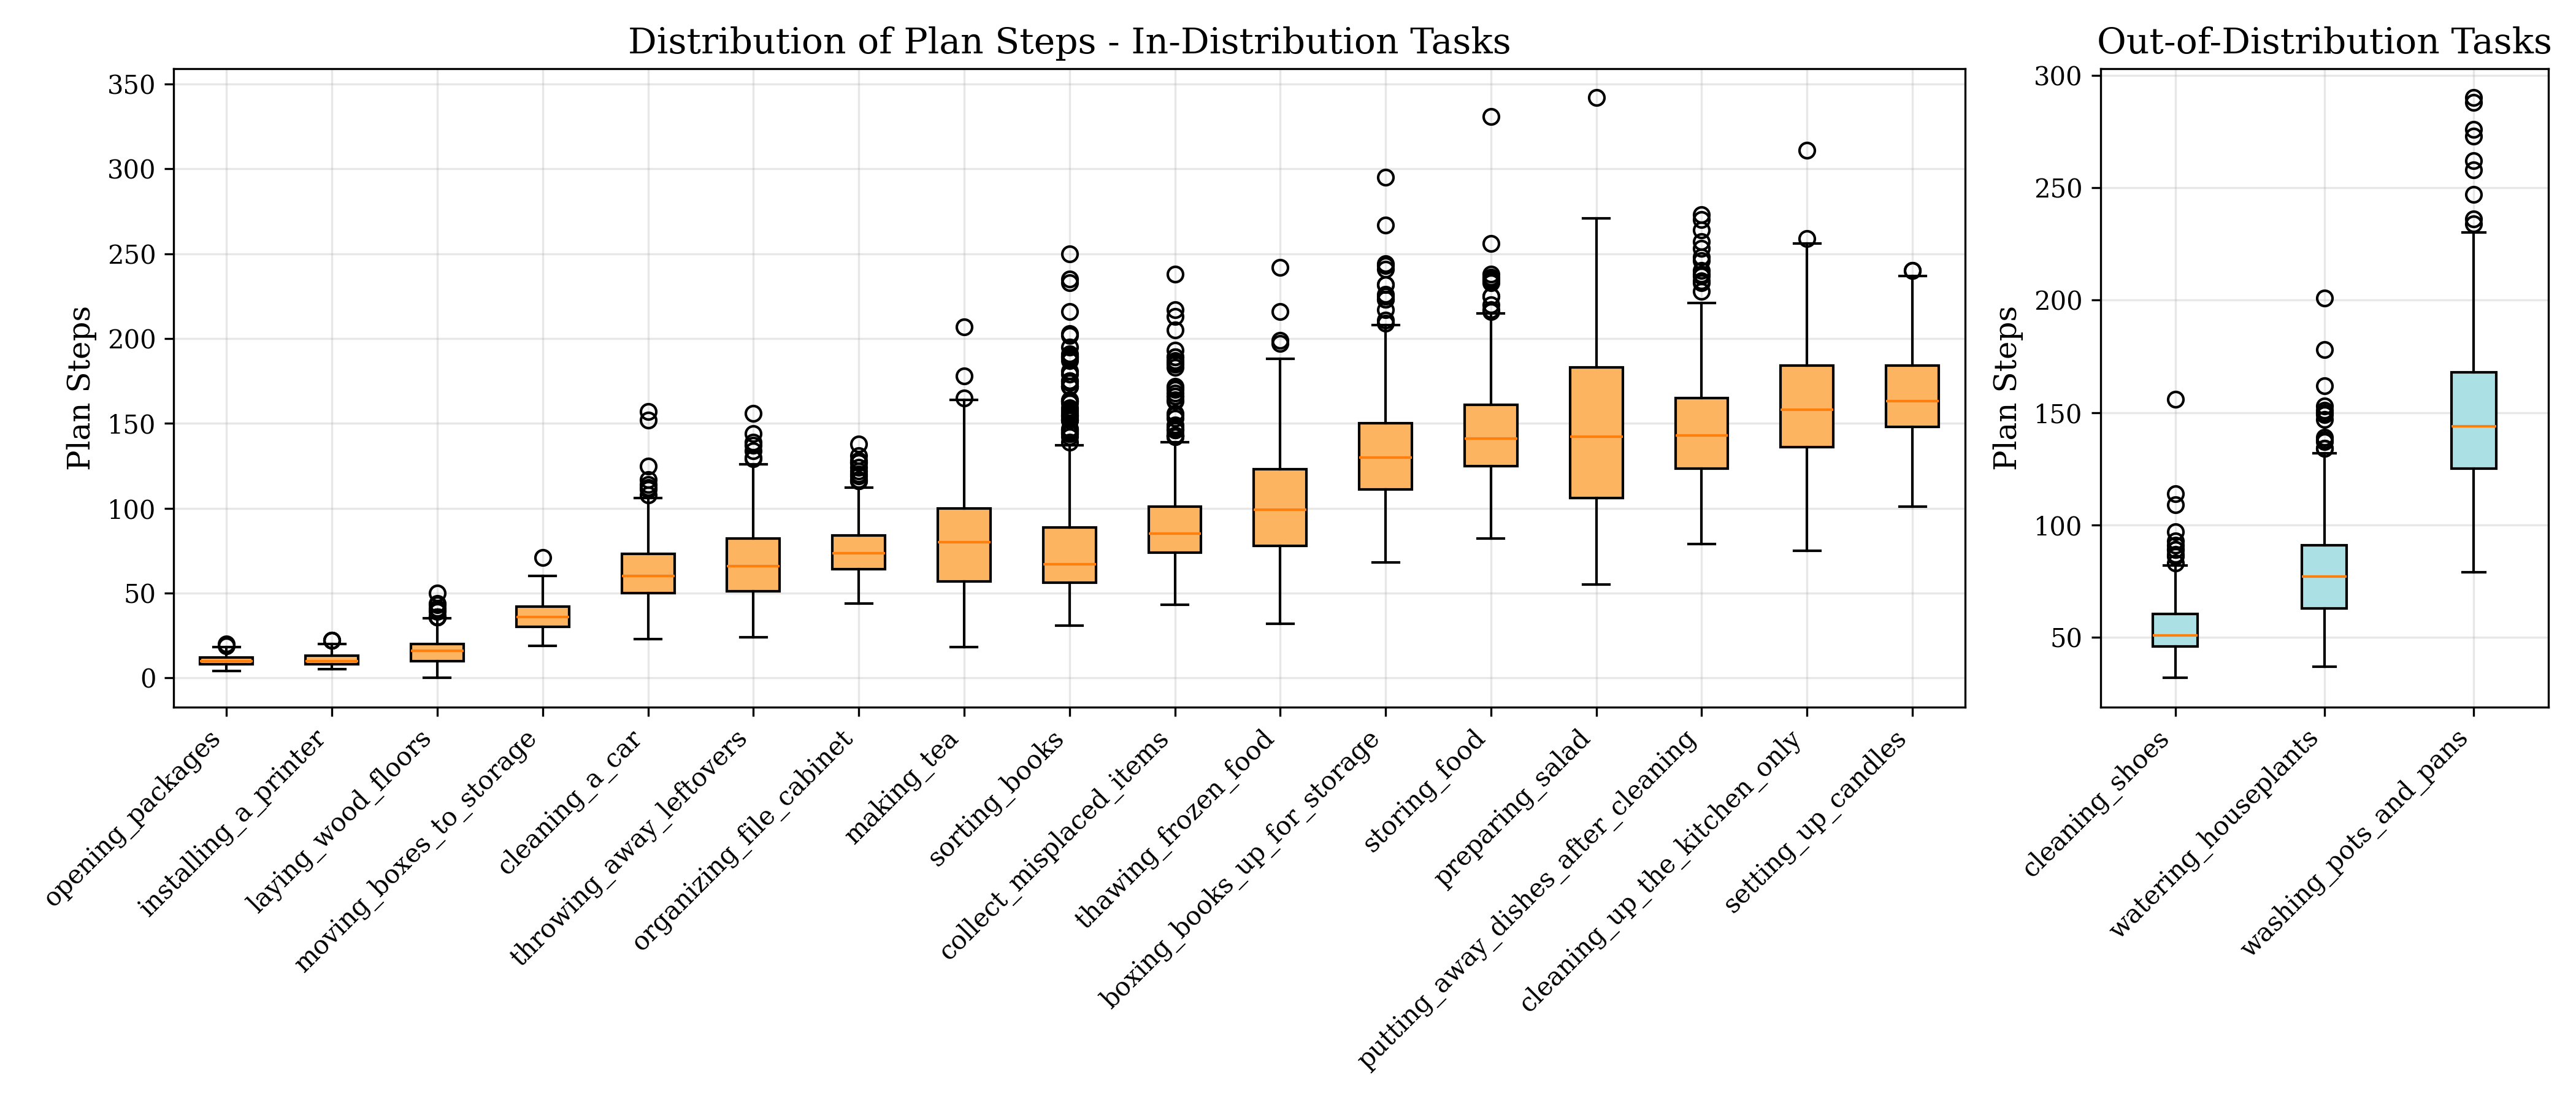
\includegraphics[width=\textwidth]{figures/plan_steps_distribution_boxplot.png}
    \caption{Distribution of reference plan steps required for tasks in \textsc{Mini-BEHAVIOR-Gran} obtained by \textsc{BWFS} classical planner.}
\end{figure*}


% ===== Fused Benchmark Task Spec Table (ID + OOD) with Goal Description =====

\begin{table*}[ht]
\small
\vspace{3mm}
\centering
\label{table:benchmark_task_spec}\scalebox{0.90}{{
\begin{tabular}{>{\centering\arraybackslash}p{4.9cm}||c|c|p{8.4cm}|c}
\toprule[0.4mm]
\cellcolor{mygray}\textbf{Task} & \cellcolor{mygray}\textbf{Split} & \cellcolor{mygray}\textbf{Class} & \cellcolor{mygray}\textbf{Goal Description} & \cellcolor{mygray}\textbf{Mean Steps} \\
\hline \hline
opening\_packages & ID & \cellcolor{green!20}\textbf{short} & Open every package. & 10.2 \\
installing\_a\_printer & ID & \cellcolor{green!20}\textbf{short} & Place a printer on a table and turn it on. & 10.6 \\
laying\_wood\_floors & ID & \cellcolor{green!20}\textbf{short} & Lay every plywood sheet on the floor, each touching at least one other sheet. & 15.9 \\
moving\_boxes\_to\_storage & ID & \cellcolor{green!20}\textbf{short} & Place every carton inside a shelf. & 36.3 \\
cleaning\_a\_car & ID & \cellcolor{green!20}\textbf{short} & Make at least one car dust-free. Place a rag and soap together inside a bucket. & 62.6 \\
throwing\_away\_leftovers & ID & \cellcolor{yellow!25}\textbf{middle} & Throw away every hamburger by placing it in a trash can. & 68.3 \\
organizing\_file\_cabinet & ID & \cellcolor{yellow!25}\textbf{middle} & Put a marker on a table and file every folder and document in a cabinet. & 75.5 \\
making\_tea & ID & \cellcolor{yellow!25}\textbf{middle} & Slice a lemon. Put a teapot on an activated stove. Keep a soaked teabag with the teapot. & 78.7 \\
sorting\_books & ID & \cellcolor{yellow!25}\textbf{middle} & Place every book and every hardback on a shelf. & 78.8 \\
collect\_misplaced\_items & ID & \cellcolor{yellow!25}\textbf{middle} & Place all gym shoes, necklaces, notebooks, and socks on a table. & 90.7 \\
thawing\_frozen\_food & ID & \cellcolor{yellow!25}\textbf{middle} & Place a date label next to a fish. Put every fish next to a sink. Set an olive next to a sink. & 101.7 \\
boxing\_books\_up\_for\_storage & ID & \cellcolor{blue!15}\textbf{long} & Place every book inside a box. & 134.4 \\
storing\_food & ID & \cellcolor{blue!15}\textbf{long} & Store every cookable item inside a cabinet. & 144.6 \\
preparing\_salad & ID & \cellcolor{blue!15}\textbf{long} & Slice all apples and tomatoes; place them on plates. Put every radish and lettuce on plates. Ensure each plate holds at least one cookable item. & 146.7 \\
putting\_away\_dishes\_after\_cleaning & ID & \cellcolor{blue!15}\textbf{long} & Put every plate inside a cabinet. & 147.7 \\
cleaning\_up\_the\_kitchen\_only & ID & \cellcolor{blue!15}\textbf{long} & Put every blender on a countertop. Refrigerate all apples and casseroles. Keep soap next to a sink. Make plates unstained and cabinets dust-free. Place each rag either beside or inside the sink. Store plates and vegetable oil in different cabinets. & 161.0 \\
setting\_up\_candles & ID & \cellcolor{blue!15}\textbf{long} & On every table, place three distinct candles on top. & 165.2 \\
\hline
cleaning\_shoes & OOD & \cellcolor{green!20}\textbf{short} & Leave a towel on the floor and make sure every shoe is unstained and dust-free. & 54.2 \\
watering\_houseplants & OOD & \cellcolor{yellow!25}\textbf{middle} & Water every potted plant until it is soaked. & 79.4 \\
washing\_pots\_and\_pans & OOD & \cellcolor{blue!15}\textbf{long} & Clean every teapot, kettle, and pan so they're unstained, then store each inside a cabinet. & 149.5 \\
\bottomrule[0.4mm]
\end{tabular}}}
\caption{Classification of tasks in \textsc{Mini-BEHAVIOR-Gran} based on the median number of plan steps, as determined by the \textsc{BWFS} planner. Tasks are categorized into short, middle, and long classes to reflect varying planning complexity based on plan length.}
\label{table:benchmark_class_based_on_plan_steps}
\end{table*}

Detailed statistics regarding the specific rule sets used for instruction generation and the resulting natural language statistics are discussed in the next section.


\section{Rule Set and Natural Language Prompt Examples For Different Tasks}
\label{app_sec:prompt_examples}

We present the rank 0 rule set for 10 over 20 household tasks in the Mini-BEHAVIOR-Gran environment. For other levels, please refer to the codebase at \url{mini-behavior-gran/mini_behavior/utils/policy_sketch/}. 

\subsection{Task 1: Laying Wood Floors}

\textbf{Features:}
\begin{itemize}[noitemsep]
    \item $H$: holding an isolated wood (plywood)
    \item $p$: distance to the nearest isolated wood
    \item $t$: distance to an arbitrary (non-held) wood we'll place next to
    \item $n$: number of isolated woods
\end{itemize}

\resizebox{\columnwidth}{!}{$
\begin{aligned}
\{\neg H, p>0, n >0\} &\mapsto \{p \downarrow, t?\} && \text{; move close to isolated wood} \\
\{\neg H, p=0, n >0\} &\mapsto \{H\} && \text{; pick up isolated wood when reachable} \\
\{H, t>0, n >0\} &\mapsto \{t\downarrow\} && \text{; move to some wood location} \\
\{H, n >0, t=0\} &\mapsto \{H?, n \downarrow, p?\} && \text{; drop the isolated wood next to other wood}
\end{aligned}
$}
\subsection{Task 2: Preparing Salad}

\textbf{Features:}
\begin{itemize}[noitemsep]
    \item $H_n$: holding a not-sliceable food
    \item $H_s$: holding a sliceable food
    \item $H_k$: holding a slicer
    \item $U$: number of sliceable food that is not sliced yet
    \item $d_p$: distance to the selected incomplete plate $p$
    \item $d_n, d_s$: distances to nearest not-sliceable / sliceable
    \item $k$: distance to a slicer (knife)
    \item $B$: selected plate $p$ complete bottom salad
    \item $n$: number of incomplete plates
    \item $nn$: number of plates that do not have bottom salad yet
\end{itemize}

\resizebox{\columnwidth}{!}{$
\noindent\textit{Acquire slicer:}
\begin{aligned}
\{U>0 , \neg H_k, k>0\} &\mapsto \{k \downarrow\} && \text{; move to slicer} \\
\{U>0 , \neg H_k, k=0\} &\mapsto \{H_k\} && \text{; hold a slicer} \\
\{U>0 , H_k, d_s > 0\} &\mapsto \{d_s \downarrow\} && \text{; move to sliceable food} \\
\{U>0 , H_k, d_s = 0\} &\mapsto \{U \downarrow, \neg H_k \} && \text{; cut sliceable food} \\
\{U=0 , H_k\} &\mapsto \{\neg H_k\} && \text{; put down slicer}
\end{aligned}
$}
\resizebox{\columnwidth}{!}{$
\noindent\textit{Place bottom salad:}
\begin{aligned}
\{n>0, U=0, nn>0, \neg B, \neg H_n, d_n>0\} &\mapsto \{d_n \downarrow\} \\
\{n>0, U=0,nn>0, \neg B, \neg H_n, d_n=0\} &\mapsto \{H_n\} \\
\{n>0, U=0,nn>0, \neg B, H_n, d_p>0\} &\mapsto \{d_p\downarrow\} \\
\{n>0, U=0, nn>0, \neg B, H_n, d_p=0\} &\mapsto \{B, nn \downarrow, \neg H_n\}
\end{aligned}
$}

\resizebox{\columnwidth}{!}{$
\noindent\textit{Handle sliceable salad:}
\begin{aligned}
\{nn=0, n>0, U=0 , \neg H_s, d_s>0\} &\mapsto \{d_s \downarrow\} && \text{; move to sliceable food} \\
\{nn=0, n>0, U=0 , \neg H_s, d_s=0\} &\mapsto \{H_s\} && \text{; pick up sliceable food} \\
\{nn=0, n>0, U=0 , H_s, d_p>0\} &\mapsto \{d_p \downarrow\} && \text{; move to the plate} \\
\{nn=0, n>0, U=0 , H_s, d_p=0\} &\mapsto \{n \downarrow, \neg H_s\} && \text{; put down sliced food}
\end{aligned}
$}

\subsection{Task 3: Cleaning Up the Kitchen Only}

\textbf{Features:}
\begin{itemize}[noitemsep]
    \item \textit{Holding flags:} $H_b$ (blender), $H_f$ (food), $H_s$ (soap), $H_r$ (rag), $H_p$ (plate), $H_o$ (vegetable oil)
    \item \textit{Distances:} $d_{ct}$ (countertop), $d_{fr}$ (fridge), $d_{si}$ (sink), $d_{c1}$ (cabinet for plate), $d_{c2}$ (cabinet for oil), $d_x$ (to object $x$)
    \item \textit{State booleans:} $\text{Open}(c)$, $\text{Tog}(s)$, $\text{Soaked}$, $\text{DustFree}(c)$, $\text{Clean}(p)$, $\text{OilIn}(c_2)$, $\text{Diff}$
    \item \textit{Counters:} $N_b$ (blenders not on countertop), $N_a$ (apples not in fridge), $N_{cas}$ (casseroles not in fridge), $N_s$ (soaps not next to sink), $N_{cab}$ (cabinets not dusted), $N_r$ (rags not next to sink), $N_{p\_clean}$ (plates not clean), $N_{oil}$ (oil not in cabinet), $N_{p\_store}$ (plates not stored), $N_{close}$ (closed furniture)
\end{itemize}

\resizebox{\columnwidth}{!}{$
\noindent\textit{Open Cabinet and Fridge:}
\begin{aligned}
\{N_{close} > 0, d_c>0\} &\mapsto \{d_c\downarrow\} && \text{; move toward closed furniture} \\
\{N_{close} > 0, d_c = 0\} &\mapsto \{N_{close}\downarrow\}
\end{aligned}
$}

\resizebox{\columnwidth}{!}{$
\noindent\textit{Oil placement:}
\begin{aligned}
\{N_{close} = 0,\neg H_o, d_{oil}>0\} &\mapsto \{d_{oil}\downarrow\} && \text{; approach oil} \\
\{N_{close} = 0,\neg H_o, d_{oil}=0\} &\mapsto \{H_o\} && \text{; pick up oil} \\
\{N_{close} = 0, H_o, N_{oil} > 0, d_{c2}>0\} &\mapsto \{d_{c2}\downarrow\} && \text{; go to cabinet } c_2 \\
\{N_{close} = 0, H_o, N_{oil} > 0, d_{c2} = 0\} &\mapsto \{N_{oil}\downarrow, \neg H_o\} && \text{; place oil in } c_2
\end{aligned}
$}

\resizebox{\columnwidth}{!}{$
\noindent\textit{Plate cleaning:}
\begin{aligned}
\{\neg \text{Tog}(s), d_{si}>0\} &\mapsto \{d_{si}\downarrow\} && \text{; toggle sink on} \\
\{\neg \text{Tog}(s), d_{si}=0\} &\mapsto \{\text{Tog}(s)\} \\
\{\neg H_r, d_{rag}>0\} &\mapsto \{d_{rag}\downarrow\} && \text{; get rag} \\
\{\neg H_r, d_{rag}=0\} &\mapsto \{H_r\} \\
\{H_r, \neg \text{Soaked}, d_{si}>0\} &\mapsto \{d_{si}\downarrow\} && \text{; soak rag} \\
\{H_r, \neg \text{Soaked}, d_{si}=0\} &\mapsto \{\text{Soaked}\} \\
\{H_r, \text{Soaked}, N_{p\_clean}>0, d_{plate}>0\} &\mapsto \{d_{plate}\downarrow\} \\
\{H_r, \text{Soaked}, N_{p\_clean}>0, d_{plate}=0\} &\mapsto \{N_{p\_clean}\downarrow, d_{plate}?\}
\end{aligned}
$}
\resizebox{\columnwidth}{!}{$
\noindent\textit{Plate placement distinct from oil:}
\begin{aligned}
\{N_{close} =0 , N_{oil}=0, N_{p\_clean} =0 ,\neg H_p, N_{p\_store}>0, d_{plate}>0\} &\mapsto \{d_{plate}\downarrow\} \\
\{N_{close} =0 , N_{oil}=0, N_{p\_clean} =0 , \neg H_p, N_{p\_store}>0, d_{plate}=0\} &\mapsto \{H_p\} \\
\{N_{close} =0 , N_{oil}=0, N_{p\_clean} =0 , H_p, N_{p\_store}>0, d_{c1}>0\} &\mapsto \{d_{c1}\downarrow\} \\
\{N_{close} =0 , N_{oil}=0, N_{p\_clean} =0 , H_p, N_{p\_store}>0, d_{c1}=0\} &\mapsto \{N_{p\_store}\downarrow, \neg H_p\}
\end{aligned}
$}

\resizebox{\columnwidth}{!}{$
\noindent\textit{Blender to countertop:}
\begin{aligned}
\{N_b > 0, \neg H_b, d_{blender}>0\} &\mapsto \{d_{blender}\downarrow\} \\
\{N_b > 0, \neg H_b, d_{blender}=0\} &\mapsto \{H_b\} \\
\{H_b, N_b>0, d_{ct}>0\} &\mapsto \{d_{ct}\downarrow\} \\
\{H_b, N_b>0, d_{ct}=0\} &\mapsto \{N_b\downarrow, \neg H_b\}
\end{aligned}
$}

\resizebox{\columnwidth}{!}{$
\noindent\textit{Apple to fridge:}
\begin{aligned}
\{N_{close} =0,\neg H_f, d_{apple}>0\} &\mapsto \{d_{apple}\downarrow\} \\
\{N_{close} =0,\neg H_f, d_{apple}=0\} &\mapsto \{H_f\} \\
\{N_{close} =0,H_f, N_a>0, d_{fr}>0\} &\mapsto \{d_{fr}\downarrow\} \\
\{N_{close} =0,H_f, N_a>0, d_{fr}=0\} &\mapsto \{N_a\downarrow, \neg H_f\}
\end{aligned}
$}

\resizebox{\columnwidth}{!}{$
\noindent\textit{Casserole to fridge:}
\begin{aligned}
\{N_{close} =0 ,\neg H_f, d_{casserole}>0\} &\mapsto \{d_{casserole}\downarrow\} \\
\{N_{close} =0 ,\neg H_f, d_{casserole}=0\} &\mapsto \{H_f\} \\
\{N_{close} =0 ,H_f, N_{cas}>0, d_{fr}>0\} &\mapsto \{d_{fr}\downarrow\} \\
\{N_{close} =0 ,H_f, N_{cas}>0, d_{fr}=0\} &\mapsto \{N_{cas}\downarrow, \neg H_f\}
\end{aligned}
$}

\resizebox{\columnwidth}{!}{$
\noindent\textit{Cabinet dusting:}
\begin{aligned}
\{\neg H_r, d_{rag}>0\} &\mapsto \{d_{rag}\downarrow\} && \text{; get rag} \\
\{\neg H_r, d_{rag}=0\} &\mapsto \{H_r\} \\
\{H_r, N_{cab}>0, d_c>0\} &\mapsto \{d_c\downarrow\} && \text{; clean cabinet} \\
\{H_r, N_{cab}>0, d_c=0\} &\mapsto \{N_{cab}\downarrow, \neg H_r\}
\end{aligned}
$}

\resizebox{\columnwidth}{!}{$
\noindent\textit{Rag near/inside sink:}
\begin{aligned}
\{N_{cab} = 0, N_{p\_clean} = 0,\neg H_r, d_{rag}>0\} &\mapsto \{d_{rag}\downarrow\} \\
\{N_{cab} = 0, N_{p\_clean} = 0,\neg H_r, d_{rag}=0\} &\mapsto \{H_r\} \\
\{N_{cab} = 0, N_{p\_clean} = 0,H_r, N_r>0, d_{si}>0\} &\mapsto \{d_{si}\downarrow\} \\
\{N_{cab} = 0, N_{p\_clean} = 0,H_r, N_r>0, d_{si}=0\} &\mapsto \{N_r\downarrow, \neg H_r\}
\end{aligned}
$}

\resizebox{\columnwidth}{!}{$
\noindent\textit{Soap next to sink:}
\begin{aligned}
\{N_{cab} = 0, N_{p\_clean} = 0,\neg H_s, d_{soap}>0\} &\mapsto \{d_{soap}\downarrow\} \\
\{N_{cab} = 0, N_{p\_clean} = 0,\neg H_s, d_{soap}=0\} &\mapsto \{H_s\} \\
\{N_{cab} = 0, N_{p\_clean} = 0,H_s, N_s>0, d_{si}>0\} &\mapsto \{d_{si}\downarrow\} \\
\{N_{cab} = 0, N_{p\_clean} = 0,H_s, N_s>0, d_{si}=0\} &\mapsto \{N_s\downarrow, \neg H_s\}
\end{aligned}
$}

\subsection{Task 4: Organizing File Cabinet}

\textbf{Features:}
\begin{itemize}[noitemsep]
    \item $H_m$: holding a marker
    \item $H_f$: holding a folder
    \item $H_d$: holding a document
    \item $p_m$: distance to the nearest marker
    \item $p_f$: distance to the nearest folder
    \item $p_d$: distance to the nearest document
    \item $p_t$: distance to a table
    \item $p_c$: distance to a valid cabinet target
    \item $N_m$: number of markers not on a table
    \item $N_f$: number of folders not in a cabinet
    \item $N_d$: number of documents not in a cabinet
    \item $N_o$: number of closed cabinets
\end{itemize}

\resizebox{\columnwidth}{!}{$
\noindent\textit{Opening Cabinet:}
\begin{aligned}
\{N_o > 0, p_c > 0\} &\mapsto \{p_c \downarrow\} && \text{; move toward a closed cabinet} \\
\{N_o > 0, p_c = 0\} &\mapsto \{N_o \downarrow\} && \text{; open the cabinet when reachable}
\end{aligned}
$}
\resizebox{\columnwidth}{!}{$
\noindent\textit{Marker task:}
\begin{aligned}
\{N_m > 0, \neg H_m, p_m > 0\} &\mapsto \{p_m \downarrow, p_t ?\} && \text{; move toward the nearest marker} \\
\{N_m > 0, \neg H_m, p_m = 0\} &\mapsto \{H_m, p_t ?\} && \text{; pick up the marker when reachable} \\
\{N_m > 0, H_m, p_t > 0\} &\mapsto \{p_t \downarrow\} && \text{; move toward a table} \\
\{N_m > 0, H_m, p_t = 0\} &\mapsto \{N_m \downarrow, \neg H_m, p_m ?\} && \text{; put marker on table}
\end{aligned}
$}
\resizebox{\columnwidth}{!}{$
\noindent\textit{Folder task:}
\begin{aligned}
\{N_f > 0, N_o = 0, \neg H_f, p_f > 0\} &\mapsto \{p_f \downarrow, p_c ?\} \\
\{N_f > 0, N_o = 0, \neg H_f, p_f = 0\} &\mapsto \{H_f, p_c ?\} \\
\{N_f > 0, N_o = 0, H_f, p_c > 0\} &\mapsto \{p_c \downarrow\} \\
\{N_f > 0, N_o = 0, H_f, p_c = 0\} &\mapsto \{N_f \downarrow, \neg H_f, p_f ?\}
\end{aligned}
$}
\resizebox{\columnwidth}{!}{$
\noindent\textit{Document task:}
\begin{aligned}
\{N_d > 0, N_o = 0, \neg H_d, p_d > 0\} &\mapsto \{p_d \downarrow, p_c ?\} \\
\{N_d > 0, N_o = 0, \neg H_d, p_d = 0\} &\mapsto \{H_d, p_c ?\} \\
\{N_d > 0, N_o = 0, H_d, p_c > 0\} &\mapsto \{p_c \downarrow\} \\
\{N_d > 0, N_o = 0, H_d, p_c = 0\} &\mapsto \{N_d \downarrow, \neg H_d, p_d ?\}
\end{aligned}
$}

\subsection{Task 5: Thawing Frozen Food}

\textbf{Features:}
\begin{itemize}[noitemsep]
    \item $H_{fish}$: holding a fish
    \item $H_{olive}$: holding an olive
    \item $H_{date}$: holding a date
    \item $p_{fish}$: distance to the nearest fish
    \item $p_{olive}$: distance to the nearest olive
    \item $p_{date}$: distance to the nearest date
    \item $p_{sink}$: distance to a sink
    \item $N_{fish}$: number of fish not next to a sink
    \item $N_{olive}$: number of olives not next to a sink
    \item $N_{date}$: number of dates not next to a fish
\end{itemize}

\resizebox{\columnwidth}{!}{$
\noindent\textit{Fish Task:}
\begin{aligned}
\{\neg H_{fish}, p_{fish} > 0\} &\mapsto \{p_{fish} \downarrow\} \\
\{\neg H_{fish}, p_{fish} = 0\} &\mapsto \{H_{fish}\} \\
\{H_{fish}, p_{sink} > 0\} &\mapsto \{p_{sink} \downarrow\} \\
\{H_{fish}, p_{sink} = 0\} &\mapsto \{N_{fish} \downarrow, \neg H_{fish}, p_{fish} ?\}
\end{aligned}
$}

\resizebox{\columnwidth}{!}{$
\noindent\textit{Olive Task:}
\begin{aligned}
\{\neg H_{olive}, p_{olive} > 0\} &\mapsto \{p_{olive} \downarrow\} \\
\{\neg H_{olive}, p_{olive} = 0\} &\mapsto \{H_{olive}\} \\
\{H_{olive}, p_{sink} > 0\} &\mapsto \{p_{sink} \downarrow\} \\
\{H_{olive}, p_{sink} = 0\} &\mapsto \{N_{olive} \downarrow, \neg H_{olive}, p_{olive} ?\}
\end{aligned}
$}

\resizebox{\columnwidth}{!}{$
\noindent\textit{Date Task:}
\begin{aligned}
\{\neg H_{date}, N_{\text{fish olive}}= 0, p_{date} > 0\} &\mapsto \{p_{date} \downarrow\} \\
\{\neg H_{date}, N_{\text{fish olive}}= 0,p_{date} = 0\} &\mapsto \{H_{date}\} \\
\{H_{date}, N_{\text{fish olive}}= 0,p_{fish} > 0\} &\mapsto \{p_{fish} \downarrow\} \\
\{H_{date}, N_{\text{fish olive}}= 0, p_{fish} = 0\} &\mapsto \{N_{date} \downarrow, \neg H_{date}, p_{date} ?\}
\end{aligned}
$}


\subsection{Task 6: Making Tea}

\textbf{Features:}
\begin{itemize}[noitemsep]
    \item $H_l$: holding a lemon
    \item $H_{knife}$: holding a knife
    \item $H_t$: holding a teapot
    \item $H_{tb}$: holding a tea bag
    \item $p_l$: distance to the nearest lemon
    \item $p_{knife}$: distance to the knife
    \item $p_t$: distance to the nearest teapot
    \item $p_{tb}$: distance to the nearest tea bag
    \item $p_s$: distance to the stove
    \item $p_{sink}$: distance to the sink
    \item $\text{is\_sliced}(\text{lemon})$: whether the lemon is sliced
    \item $\text{is\_toggled}(\text{stove})$: whether the stove is toggled on
    \item $\text{is\_toggled}(\text{sink})$: whether the sink is toggled on
    \item $\text{is\_soaked}(\text{tea\_bag})$: whether the tea bag is soaked
    \item $\text{atsamelocation}(\text{tea\_bag}, \text{teapot})$: tea bag at same location as teapot
    \item $\text{onTop}(\text{teapot}, \text{stove})$: teapot on stove
\end{itemize}

\resizebox{\columnwidth}{!}{$
\noindent\textit{Toggle stove:}
\begin{aligned}
\{\neg \text{is\_toggled}(\text{stove}), p_s > 0\} &\mapsto \{p_s \downarrow\} \\
\{\neg \text{is\_toggled}(\text{stove}), p_s = 0\} &\mapsto \{\text{is\_toggled}(\text{stove})\}
\end{aligned}
$}
\resizebox{\columnwidth}{!}{$
\noindent\textit{Slice lemon:}
\begin{aligned}
\{\neg H_{knife}, p_{knife} > 0, \neg \text{is\_sliced}(\text{lemon})\} &\mapsto \{p_{knife} \downarrow\} \\
\{\neg H_{knife}, p_{knife} = 0, \neg \text{is\_sliced}(\text{lemon})\} &\mapsto \{H_{knife}\} \\
\{H_{knife}, \neg \text{is\_sliced}(\text{lemon}), p_{l} > 0\} &\mapsto \{p_{l} \downarrow\} \\
\{H_{knife}, \neg \text{is\_sliced}(\text{lemon}), p_{l} = 0\} &\mapsto \{\text{is\_sliced}(\text{lemon})\} \\
\{H_{knife}, \text{is\_sliced}(\text{lemon})\} &\mapsto \{\neg H_{knife}, p_{knife} ?\}
\end{aligned}
$}
\resizebox{\columnwidth}{!}{$
\noindent\textit{Handle teapot:}
\begin{aligned}
\{\neg \text{atsameloc}(\text{tb}, \text{tp}), \neg \text{onTop}(\text{tp}, \text{st}), \neg H_t, p_t > 0\} &\mapsto \{p_t \downarrow\} \\
\{\neg \text{atsameloc}(\text{tb}, \text{tp}), \neg \text{onTop}(\text{tp}, \text{st}), \neg H_t, p_t = 0\} &\mapsto \{H_t\} \\
\{\neg \text{atsameloc}(\text{tb}, \text{tp}), \neg \text{onTop}(\text{tp}, \text{st}), H_t, p_s > 0\} &\mapsto \{p_s \downarrow\} \\
\{\neg \text{atsameloc}(\text{tb}, \text{tp}), \neg \text{onTop}(\text{tp}, \text{st}), H_t, p_s = 0\} &\mapsto \{\text{onTop}(\text{tp}, \text{st}), \neg H_t, p_t ?\} \\
\{\neg \text{atsameloc}(\text{tb}, \text{tp}), \text{onTop}(\text{tp}, \text{st}), \neg H_{tb}, p_{tb} > 0\} &\mapsto \{p_{tb} \downarrow\} \\
\{\neg \text{atsameloc}(\text{tb}, \text{tp}), \text{onTop}(\text{tp}, \text{st}), \neg H_{tb}, p_{tb} = 0\} &\mapsto \{H_{tb}\} \\
\{\neg \text{atsameloc}(\text{tb}, \text{tp}), \text{onTop}(\text{tp}, \text{st}), H_{tb}, p_t > 0\} &\mapsto \{p_t \downarrow\} \\
\{H_{tb}, \neg \text{atsameloc}(\text{tb}, \text{tp}), \text{onTop}(\text{tp}, \text{st}), p_t = 0\} &\mapsto \{\text{atsameloc}(\text{tb}, \text{tp}), \neg H_{tb}, p_{tb} ?\}
\end{aligned}
$}

\subsection{Task 7: Opening Packages}

\textbf{Features:}
\begin{itemize}[noitemsep]
    \item $p$: distance to the nearest package
    \item $N$: number of unopened packages
\end{itemize}

\resizebox{\columnwidth}{!}{$
\begin{aligned}
\{N > 0, p > 0\} &\mapsto \{p \downarrow\} && \text{; move toward the nearest unopened package} \\
\{N > 0, p = 0\} &\mapsto \{N \downarrow\} && \text{; open the package when reachable}
\end{aligned}
$}

\subsection{Task 8: Boxing Books Up for Storage}

\textbf{Features:}
\begin{itemize}[noitemsep]
    \item $H$: holding an unboxed book
    \item $p$: distance to the nearest unboxed book
    \item $b$: distance to a valid box target
    \item $N$: number of unboxed books
\end{itemize}

\resizebox{\columnwidth}{!}{$
\begin{aligned}
\{\neg H, p > 0\} &\mapsto \{p \downarrow, b ?\} && \text{; move toward the nearest unboxed book} \\
\{\neg H, p = 0\} &\mapsto \{H\} && \text{; pick up the book when reachable} \\
\{H, N > 0, b > 0\} &\mapsto \{b \downarrow\} && \text{; move toward a chosen box spot} \\
\{H, N > 0, b = 0\} &\mapsto \{\neg H, N \downarrow, p ?\} && \text{; place the book into the box}
\end{aligned}
$}

\subsection{Task 9: Collect Misplaced Items}

\textbf{Features:}
\begin{itemize}[noitemsep]
    \item $H_s$: holding a gym shoe
    \item $H_n$: holding a necklace
    \item $H_b$: holding a notebook
    \item $H_k$: holding a sock
    \item $p_s$: distance to the nearest gym shoe
    \item $p_n$: distance to the nearest necklace
    \item $p_b$: distance to the nearest notebook
    \item $p_k$: distance to the nearest sock
    \item $p_t$: distance to a table
    \item $N_s$: number of gym shoes not on a table
    \item $N_n$: number of necklaces not on a table
    \item $N_b$: number of notebooks not on a table
    \item $N_k$: number of socks not on a table
\end{itemize}

\resizebox{\columnwidth}{!}{$
\noindent\textit{Gym shoe task:}
\begin{aligned}
\{\neg H_s, N_s > 0, p_s > 0\} &\mapsto \{p_s \downarrow, p_t ?\} \\
\{\neg H_s, N_s > 0, p_s = 0\} &\mapsto \{H_s, p_t ?\} \\
\{H_s, N_s > 0, p_t > 0\} &\mapsto \{p_t \downarrow\} \\
\{H_s, N_s > 0, p_t = 0\} &\mapsto \{N_s \downarrow, \neg H_s, p_s ?\}
\end{aligned}
$}
\resizebox{\columnwidth}{!}{$
\noindent\textit{Necklace task:}
\begin{aligned}
\{\neg H_n, N_n > 0, p_n > 0\} &\mapsto \{p_n \downarrow, p_t ?\} \\
\{\neg H_n, N_n > 0, p_n = 0\} &\mapsto \{H_n, p_t ?\} \\
\{H_n, N_n > 0, p_t > 0\} &\mapsto \{p_t \downarrow\} \\
\{H_n, N_n > 0, p_t = 0\} &\mapsto \{N_n \downarrow, \neg H_n, p_n ?\}
\end{aligned}
$}
\resizebox{\columnwidth}{!}{$
\noindent\textit{Notebook task:}
\begin{aligned}
\{\neg H_b, N_b > 0, p_b > 0\} &\mapsto \{p_b \downarrow, p_t ?\} \\
\{\neg H_b, N_b > 0, p_b = 0\} &\mapsto \{H_b, p_t ?\} \\
\{H_b, N_b > 0, p_t > 0\} &\mapsto \{p_t \downarrow\} \\
\{H_b, N_b > 0, p_t = 0\} &\mapsto \{N_b \downarrow, \neg H_b, p_b ?\}
\end{aligned}
$}
\resizebox{\columnwidth}{!}{$
\noindent\textit{Sock task:}
\begin{aligned}
\{\neg H_k, N_k > 0, p_k > 0\} &\mapsto \{p_k \downarrow, p_t ?\} \\
\{\neg H_k, N_k > 0, p_k = 0\} &\mapsto \{H_k, p_t ?\} \\
\{H_k, N_k > 0, p_t > 0\} &\mapsto \{p_t \downarrow\} \\
\{H_k, N_k > 0, p_t = 0\} &\mapsto \{N_k \downarrow, \neg H_k, p_k ?\}
\end{aligned}
$}

\subsection{Task 10: Putting Away Dishes After Cleaning}

\textbf{Features:}
\begin{itemize}[noitemsep]
    \item $H$: holding a plate
    \item $p$: distance to the nearest plate
    \item $b$: distance to a valid cabinet target
    \item $N$: number of unboxed plates
    \item $\text{is\_opened}$: whether the cabinet is opened
\end{itemize}

\resizebox{\columnwidth}{!}{$
\begin{aligned}
\{\neg \text{is\_opened}, b > 0\} &\mapsto \{b \downarrow\} && \text{; move toward the cabinet} \\
\{\neg \text{is\_opened}, b = 0\} &\mapsto \{\text{is\_opened}\} && \text{; open the cabinet when reachable} \\
\{\neg H, N > 0, p > 0, \text{is\_opened}\} &\mapsto \{p \downarrow, b ?\} \\
\{\neg H, N > 0, p = 0, \text{is\_opened}\} &\mapsto \{H, b ?\} \\
\{H, N > 0, b > 0, \text{is\_opened}\} &\mapsto \{b \downarrow\} \\
\{H, N > 0, b = 0, \text{is\_opened}\} &\mapsto \{\neg H, N \downarrow, p ?\}
\end{aligned}
$}



\subsection{Instruction Generation Statistics} We used a template-based generator to translate the symbolic rule sets into natural language instructions, ensuring alignment with the VLA's training data format. Table \ref{tab:instruction_stats} presents the summary statistics for the generated instructions across the three granularity levels.

\begin{table*}[t] 
\centering 
\caption{Statistics of generated natural language instructions across granularity levels.} 
\label{tab:instruction_stats} 
\resizebox{\textwidth}{!}{% 
\begin{tabular}{l|c|c|c|c|c|c|c|c}
\toprule 
\textbf{Granularity} & \textbf{Count} & \textbf{Avg Length} & \textbf{Std Length} & \textbf{Min} & \textbf{Max} & \textbf{Unique Tokens} & \textbf{TTR} & \textbf{Avg Sent. Length} \\ 
 & & \textbf{(words)} & & & & & \textbf{(Type-Token Ratio)} & \\ 
\midrule
\textbf{Fine (F)} & 1636 & 41.12 & 11.36 & 19 & 87 & 140 & 0.0021 & 41.12 \\ 
\textbf{Medium (M)} & 859 & 38.62 & 12.76 & 22 & 81 & 108 & 0.0033 & 38.62 \\ 
\textbf{Coarse (C)} & 587 & 33.60 & 13.39 & 22 & 95 & 94 & 0.0048 & 33.60 \\ 
\bottomrule 
\end{tabular}% 
} 
\end{table*}



\section{Implementation Details}
\label{app_sec:implementation_details}

\subsection{Model Architecture}

Our policy is built upon the OpenVLA architecture \citep{DBLP:conf/corl/KimPKXB0RFSVKBT24}. Specifically, we utilize the Prismatic-7B backbone \citep{DBLP:conf/icml/Karamcheti0BLKS24}, which integrates a frozen Llama-2-7B language model with fused visual features. The visual encoder consists of a dual-stream setup combining SigLIP (for semantic understanding) and DINOv2 (for fine-grained spatial geometry) \citep{DBLP:conf/iccv/ZhaiM0B23,DBLP:journals/tmlr/OquabDMVSKFHMEA24}.

\subsection{Training Configuration}

We fine-tune the model using Low-Rank Adaptation (LoRA) on the language model backbone, keeping the visual encoders frozen. All training setting variants (Pure, Centroid, Axial) share the same underlying training hyperparameters to ensure fair comparison.

Hardware and Duration: Training was conducted on a single node equipped with 8$\times$ NVIDIA A100 GPUs. A standard training run for 100,000 steps took approximately 23 hours to complete.

Table \ref{tab:hyperparameters} summarizes the core hyperparameters used across our experiments.

\begin{table}[H]
\centering
\caption{Hyperparameters for OpenVLA fine-tuning on \textsc{Mini-BEHAVIOR-Gran}.}
\label{tab:hyperparameters}
\resizebox{\columnwidth}{!}{%
\begin{tabular}{l|c}
\toprule
\textbf{Hyperparameter} & \textbf{Value} \\
\midrule
Base Model & Prismatic-7B (Llama-2) \\
Visual Encoders & SigLIP + DINOv2 \\
Parameter Efficient Tuning & LoRA (Rank $r=32$) \\
Compute Hardware & 8$\times$ NVIDIA A100 \\
Training Duration & $\sim$23 hours \\
Optimization Steps & 100,000 \\
Steps Before Decay & 80,000 \\
Learning Rate & $2.5 \times 10^{-4}$ \\
Batch Size (per GPU) & $7 - 8$ \\
\bottomrule
\end{tabular} %
}
\end{table}

We also train a lightweight VLM predictor to quantify instruction predictability via perplexity. The model is fine-tuned using Low-Rank Adaptation (LoRA) on the Qwen3-VL-4B-Instruct backbone, with vision encoders frozen to preserve visual grounding capabilities established during pretraining. All models are trained on \textsc{Mini-BEHAVIOR-Gran} instruction and image training data pairs, with training and evaluation splits maintained consistently across experiments. Hardware and Duration: Training was conducted on a single node equipped with 4$\times$ NVIDIA RTX 5090 GPUs. Each training run for 2 epochs. Table \ref{tab:qwen_hyperparameters} summarizes the core hyperparameters used for VLM predictor training.

\begin{table}[H]
\centering
\caption{Hyperparameters for Qwen3-VL-4B-Instruct fine-tuning on \textsc{Mini-BEHAVIOR-Gran} (High-domain).}
\label{tab:qwen_hyperparameters}
\resizebox{\columnwidth}{!}{%
\begin{tabular}{l|c}
\toprule
\textbf{Hyperparameter} & \textbf{Value} \\
\midrule
Base Model & Qwen3-VL-4B-Instruct \\
Visual Encoders & Frozen (Qwen3-VL native) \\
Parameter Efficient Tuning & LoRA (Rank $r=64$, $\alpha=128$) \\
LoRA Target Modules & All linear layers \\
Compute Hardware & 4$\times$ NVIDIA RTX 5090 \\
Training Epochs & 2 \\
Learning Rate & $1.0 \times 10^{-5}$ \\
Learning Rate Scheduler & Cosine with 10\% warmup \\
Batch Size (per GPU) & 32 \\
Seed & [42,50,60] \\
Gradient Accumulation Steps & 1 \\
DeepSpeed Strategy & Zero-2 \\
\bottomrule
\end{tabular} %
}
\end{table}



\section{Additional Experimental Results}
\label{app_sec:additional_experimental_results}

This section provides additional detailed per-task performance breakdowns, and failure mode distributions.

\subsection{Detailed Task Performance} 

Figure \ref{fig:per_task_success_rate} details the success rates across all 20 tasks in the benchmark. We see some tasks are too difficult to solve and thus low across all instruction granularity. And then we also see the U shape trends in most tasks, showing the same phenomenon we discussed in \textbf{(Q1)} that both very fine and very coarse instructions are easier for VLA to follow.


\begin{figure*}[t]
    \centering
    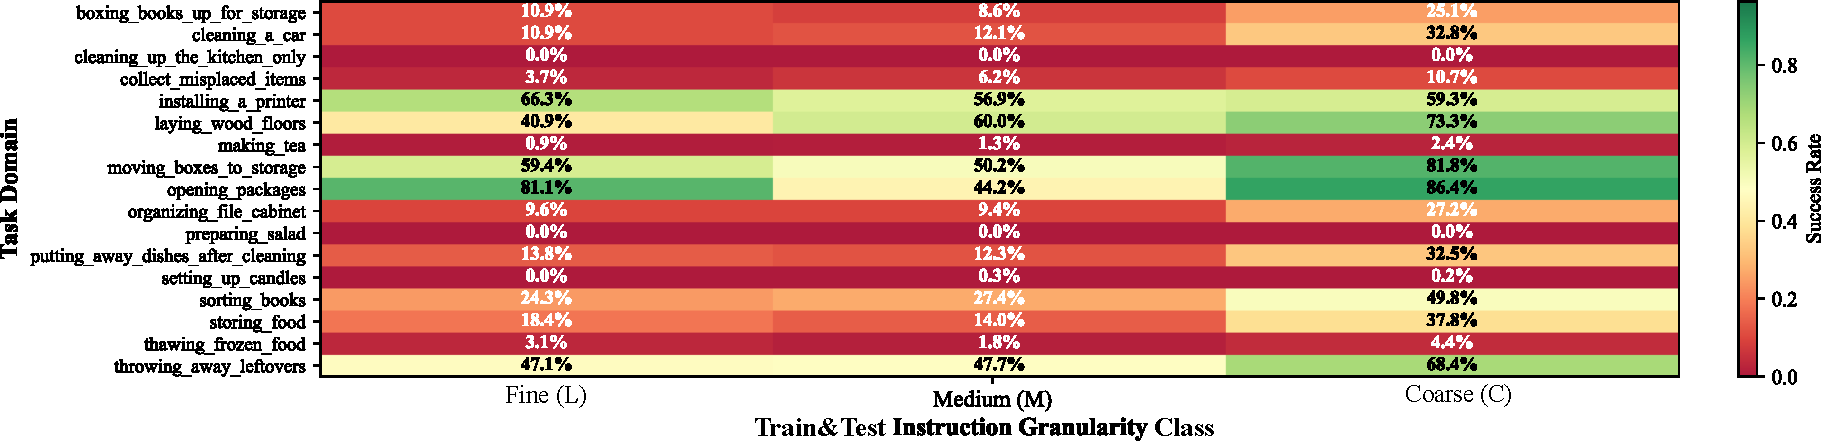
\includegraphics[width=\linewidth]{figures/q1_task_success_rate.pdf}
    \caption{Detailed per-task success rates.}
    \label{fig:per_task_success_rate}
\end{figure*}

\subsection{Detailed Attention Analysis Table}
\label{app_sec:full_attention_analysis_table}

We quantify the internal information-gathering behavior of Vision-Language-Action (VLA) models by analyzing the \textbf{attention weight distribution of the action tokens}. In these architectures, the action tokens serve as the terminal query point; their attention allocation reveals which input modalities (vision vs. language) the model prioritizes at different stages of its internal processing hierarchy.

\subsubsection{Input Sequence Formalization}
The input sequence $\mathcal{S}$ is composed of visual patches, linguistic tokens, and action tokens. Given a single sample, the sequence layout is defined as:
\begin{equation}
    \mathcal{S} = [ \texttt{BOS}, \underbrace{v_1, \dots, v_P}_{\text{vision}}, \underbrace{t_1, \dots, t_T}_{\text{text}}, \underbrace{a_1, \dots, a_A}_{\text{action}}, \texttt{EOS} ]
\end{equation}
where $P$ is the number of visual patch tokens, $T$ is the number of text tokens (comprising both prompt prefix and task instruction), and $A$ is the number of action tokens (where $A = d_{\text{action}} \times \text{chunk size}$). 

For analysis, we exclude the $[\texttt{BOS}]$ and $[\texttt{EOS}]$ boundary tokens. For each layer $\ell \in \{1, \dots, L\}$, we extract the trimmed attention tensor:
\begin{equation}
    \mathbf{A}^{(\ell)} \in \mathrm{R}^{H \times (P+T+A) \times (P+T+A)}
\end{equation}

\subsubsection{Partitioning of Semantic Regions}
To distinguish between general linguistic context and specific task instructions, we partition the key dimension (columns) of $\mathbf{A}^{(\ell)}$ into four non-overlapping semantic regions:

\textit{Note: For models utilizing compressed instruction patches, the compressed embeddings are mapped to the Dynamic Text category to ensure functional consistency across architectures.}

\subsubsection{Quantitative Measurement}
For each layer $\ell$ and head $h$, we isolate the \textbf{action-to-key} sub-matrix $\mathbf{A}^{(\ell)}_{h,\text{action} \to \text{key}} \in \mathrm{R}^{A \times (P+T+A)}$. The mean attention mass allocated to a specific region $R = [r_{\text{start}}, r_{\text{end}})$ is computed by summing weights across the region and averaging over the $A$ action tokens:
\begin{equation}
    \text{attn}_h(R) = \frac{1}{A} \sum_{i=1}^{A} \sum_{j=r_{\text{start}}}^{r_{\text{end}}-1} \mathbf{A}^{(\ell)}_{h,\text{action} \to \text{key}}[i, j]
\end{equation}

\subsubsection{Aggregation and Normalization}
To derive a layer-wise modality reliance score, we perform the following:
\begin{enumerate}
    \item \textbf{Head Averaging}: $\text{attn}(R) = \frac{1}{H} \sum_{h=1}^{H} \text{attn}_h(R)$.
    \item \textbf{Sample Mean}: Values are averaged across all samples within a specific granularity-model pair.
    \item \textbf{Simplex Normalization}: The final regional shares $\hat{a}_R$ are normalized such that $\sum_{R} \hat{a}_R = 1$.
\end{enumerate}

\subsubsection{Statistical Trend Hypothesis Testing}
We define three binary indicators to test the \textbf{Shallow Grounding Hypothesis} layer-wise:
\begin{itemize}
    \item \textbf{T1 (Lang $\uparrow$)}: $\hat{a}_{\text{text}}(\text{Medium}) > \hat{a}_{\text{text}}(\text{Fine})$
    \item \textbf{T2 (Lang $\downarrow$)}: $\hat{a}_{\text{text}}(\text{Medium}) > \hat{a}_{\text{text}}(\text{Coarse})$
    \item \textbf{T3 (Vis $\uparrow$)}: $\hat{a}_{\text{vis}}(\text{Coarse}) > \hat{a}_{\text{vis}}(\text{Medium})$
\end{itemize}
We assess the significance of these trends across $N=32$ layers using a \textbf{one-sided Binomial test} ($H_0: p=0.5$). Significance is reported as $^{*}p < 0.05$ and $^{**}p < 0.01$. Confidence intervals for proportions are calculated using the \textbf{Clopper-Pearson} method. The full statistical breakdown is presented in \Cref{tab:full_stats_appendix}.

\begin{table*}[h]
\centering
\small
\begin{tabular}{ll cccc c}
\toprule
\textbf{Model} & \textbf{Trend} & \textbf{k/N} & \textbf{Prop.} & \textbf{95\% CI} & \textbf{$H_0$} & \textbf{$p$-value} \\
\midrule
Autoregressive     & T1 & 25/32 & 78.1\% & [0.600, 0.907] & 50.0\% & 0.0011 \\
                   & T2 & 4/32  & 12.5\% & [0.035, 0.290] & 50.0\% & 1.0000 \\
                   & T3 & 21/32 & 65.6\% & [0.468, 0.814] & 50.0\% & 0.1102 \\
\midrule
Parallel Decoding  & T1 & 5/32  & 15.6\% & [0.053, 0.328] & 50.0\% & 1.0000 \\
                   & T2 & 9/32  & 28.1\% & [0.137, 0.467] & 50.0\% & 0.9965 \\
                   & T3 & 5/32  & 15.6\% & [0.053, 0.328] & 50.0\% & 1.0000 \\
\midrule
Discrete Diffusion & T1 & 17/32 & 53.1\% & [0.347, 0.709] & 50.0\% & 0.4300 \\
                   & T2 & 23/32 & 71.9\% & [0.533, 0.863] & 50.0\% & 0.0100 \\
                   & T3 & 24/32 & 75.0\% & [0.566, 0.885] & 50.0\% & 0.0035 \\
\bottomrule
\end{tabular}
\caption{Detailed statistical analysis of layer-wise attention trends across architectures. P-values are calculated using a one-sided Binomial test against a null hypothesis ($H_0$) of 0.5. Confidence intervals (CI) are calculated at the 95\% level.}
\label{tab:full_stats_appendix}
\end{table*}

\subsection{Failure Analysis} 
Figure \ref{fig:failure_type_dist_by_width} presents the distribution of failure types across varying instruction widths. It confirms that low width encounters regression failures more frequently, while high width predominantly leads to stagnation failures. This aligns with our earlier observations in \Cref{fig:q4_failure_modes} regarding the distinct failure modes associated with different instruction granularities. Agent failure distributions bifurcate strictly with width. Low-width, long-horizon tasks predominantly suffer from \emph{regression}: the agent violates previously satisfied fluents and cycles back to prior states, reflecting subgoal serialization failures. High-width tasks ($w \ge 3$), by contrast, exhibit \emph{stagnation}: the agent freezes, unable to resolve concurrent feature dependencies ($O(|\Phi|^w)$) required to initiate a valid state transition. This dichotomy mirrors the width-based complexity landscape.

\begin{figure}[H]
    \centering
    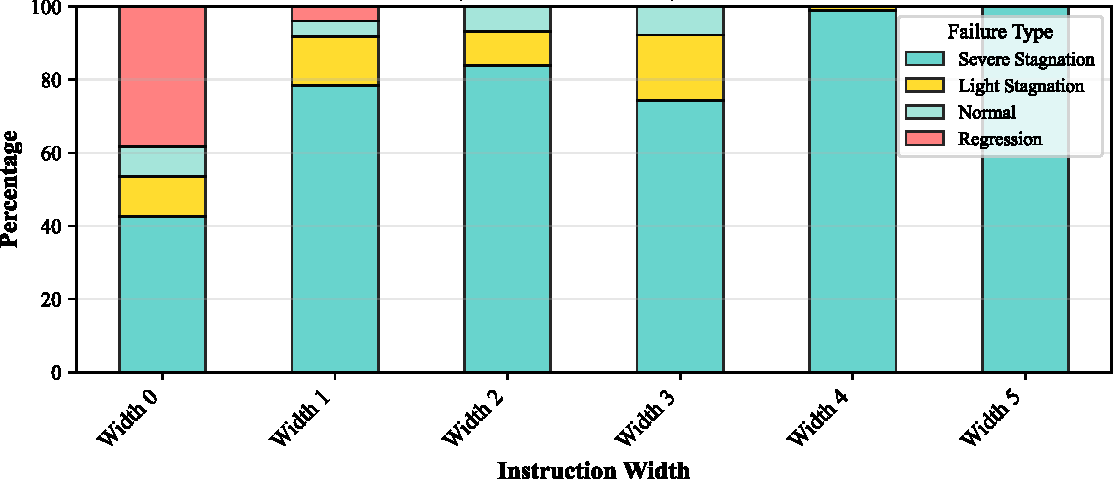
\includegraphics[width=\linewidth]{figures/q4_failure_type_dist_by_width.pdf}
    \caption{Failure type distribution across instruction widths.}
    \label{fig:failure_type_dist_by_width}
\end{figure}

\begin{figure}[H]
    \centering
    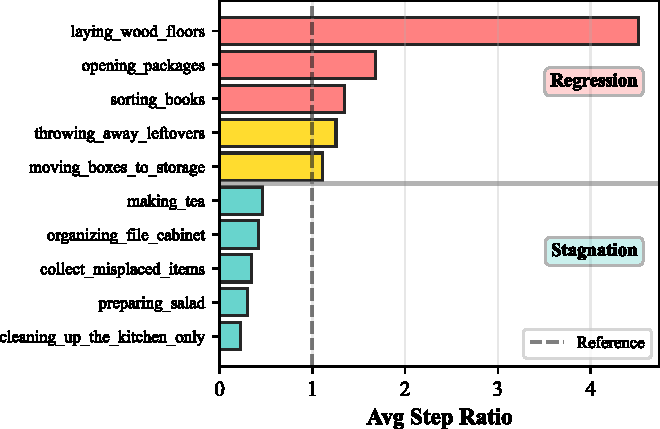
\includegraphics[width=\linewidth, keepaspectratio]{figures/q4_failure_type_extreme_task_example.pdf}
    \captionof{figure}{Low-width but long task horizon (e.g., laying woods) tends to cause regression, while high-width stagnates.}
    \label{fig:q4_failure_modes}
\end{figure}

\subsection{More Plots for Width vs. Other Linguistic Heuristics as Metric for Language Grounding Complexity}

As shown in the correlation heatmap \Cref{fig:correlation_heatmap}, $w$ is the only metric that maintains a stable negative correlation with Success Rate across all horizons. In contrast, surface metrics like Token Count and Entity Count exhibit near-zero or even positive correlations in shorter horizons (e.g., $r=0.09$ for 1-5 steps). This confirms the Complexity Paradox: while longer, more detailed instructions (higher token/entity counts) could actually provide helpful guidance that improves SR, increasing the latent planning width ($w$) invariably degrades performance.

\begin{figure}[H]
    \centering
    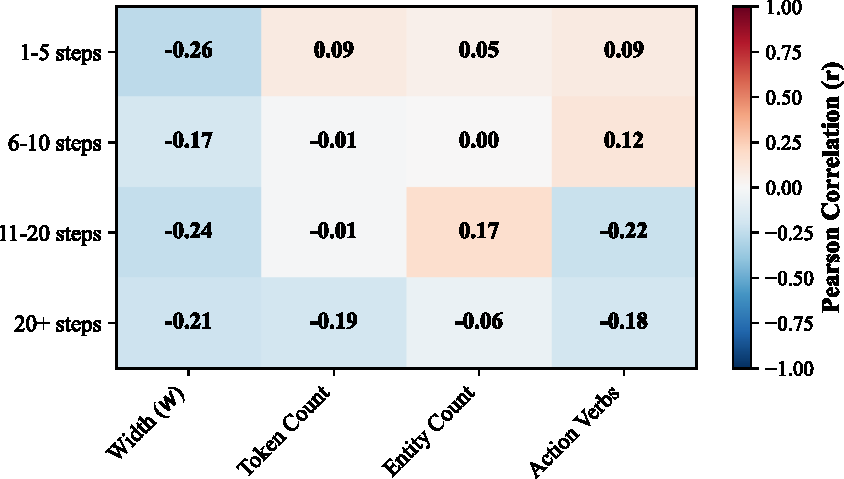
\includegraphics[width=\linewidth]{figures/q8_correlation_heatmap.pdf}
    \caption{Correlation heatmap between instruction width and other linguistic heuristics.}
    \label{fig:correlation_heatmap}
\end{figure}

Similarly, the consistency analysis in \Cref{fig:consistency_comparison} shows that $w$ possesses the lowest standard deviation ($\sigma=0.033$), indicating its predictive reliability is invariant to task horizons. Surface metrics, particularly Action Verbs ($\sigma=0.155$), are highly volatile. It also shows that $w$ provides the highest mean predictive power ($|r|=0.220$), more than doubling the predictive strength of Token Count ($0.076$) or Entity Count ($0.072$).

\begin{figure}[H]
    \centering
    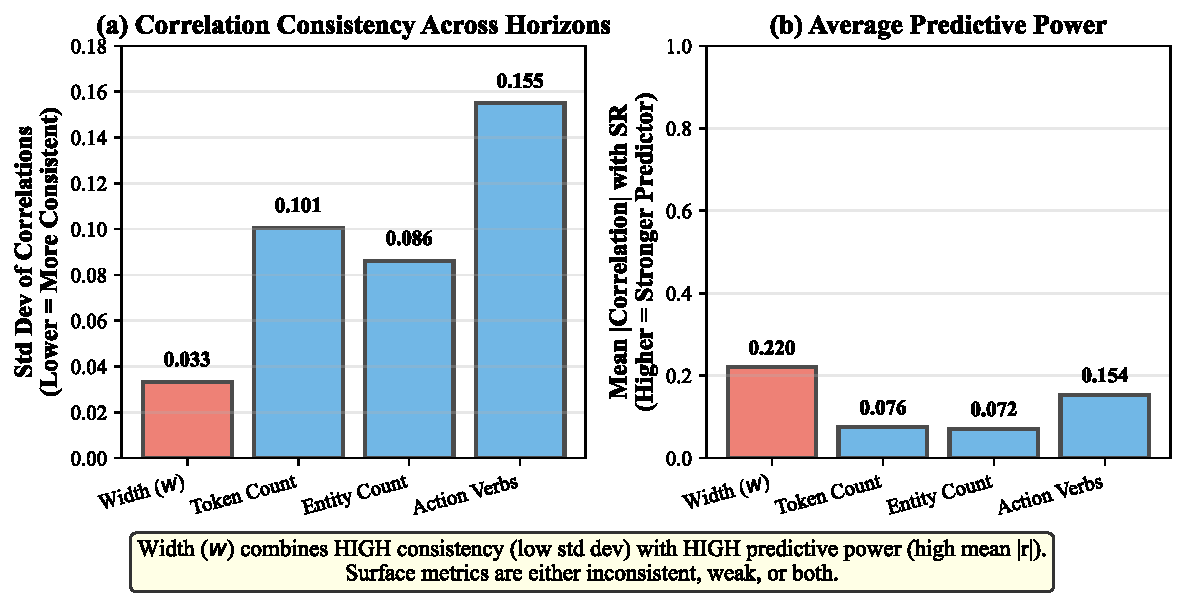
\includegraphics[width=\linewidth]{figures/q8_consistency_comparison.pdf}
    \caption{Consistency comparison between instruction width and other linguistic heuristics.}
    \label{fig:consistency_comparison}
\end{figure}

% \subsection{VLA Transformer Attention Weight Visualization}

% \begin{figure}[H]
%     \centering
%     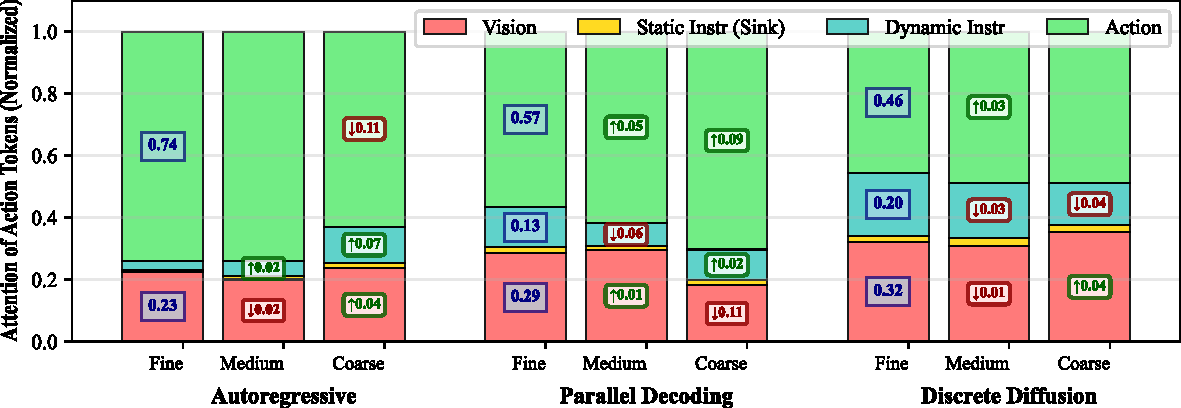
\includegraphics[width=\linewidth]{figures/q6_compare_baseline_models_attention_dist.pdf}
%     \captionof{figure}{Attention from action tokens. Self-attention dominates, followed by vision; No clear trend across granularity levels.}
%     \label{fig:attention_distribution_baseline_models}
% \end{figure}

% Attention analysis (\Cref{fig:attention_distribution_baseline_models}) reveals there is no obvious reduction in language-token attention. This suggests that in VLA architectures, maintained attention weights do not necessarily equate to language grounding, highlighting a complex dynamic that requires future investigation. 

% Nevertheless, a closer inspection of the attention distributions reveals distinct architectural behaviors and compensatory mechanisms.

% \paragraph{Autoregressive Models (Compensatory Reading).} Autoregressive generation exhibits a heavy baseline reliance on historical action tokens (accounting for $0.74$ of normalized attention in the Fine setting). Interestingly, when presented with Coarse instructions, attention to the dynamic instruction increases ($\uparrow 0.07$) while action attention decreases ($\downarrow 0.11$). This suggests a compensatory mechanism: as the rule width $w$ increases and immediate subgoals disappear, the model attempts to ground more heavily on the language prompt to search for clues.

% \paragraph{Parallel Decoding (Attending more on action modality).} This architecture demonstrates a stark multimodal decoupling under coarse instructions. The attention paid to visual tokens drops significantly ($\downarrow 0.11$) in the Coarse setting, accompanied by an increased reliance on generated action tokens ($\uparrow 0.09$). This could imply that without detailed instruction guidance at each step, parallel decoding intend to trust more on action history to decide the next actions, showing a different strategy from autoregressive models.

% \paragraph{Discrete Diffusion (Structural Stability).} Diffusion models exhibit the most balanced attention distribution, maintaining the highest baseline attention to both dynamic instructions ($0.20$) and visual features ($0.32$). Notably, this distribution remains remarkably rigid regardless of instruction granularity (with fluctuations bounded within $\pm 0.04$).


\subsection{Sample Generated Instructions by Granularity} \label{app_sec:sample_instructions}

To illustrate the qualitative differences between granularity levels, we provide five random samples for each category below. Note how Low (L) granularity explicitly specifies navigation and preconditions (e.g., move toward,'' not yet at''), while High (H) granularity focuses almost exclusively on the final state change (e.g., ``reduce the count of...''), shown in Table~\ref{tab:sample_instructions}.

\begin{table*}[ht]
\centering
\begin{minipage}{\textwidth}

\noindent\textbf{Fine Granularity (F) Samples}
\begin{tcolorbox}[colback=green!5, colframe=green!40!black]
\small
\begin{enumerate}
    \item At step 11: When the count of uncleaned plate is above 0, not yet at sink 0 and sink is off, please try to move toward sink 0.
    \item At step 8: When not yet at soap 0, not holding soap 0, the count of unwiped car is 0 and the count of rag not inside bucket is 0, please try to move toward soap 0.
    \item At step 27: When the count of chip and oatmeal sugar and vegetable oil not inside cabinet is above 0, you are at oatmeal 1 and not holding oatmeal 1, please pick up oatmeal 1.
    \item At step 15: When the count of plate not inside cabinet is above 0, you are at plate 3, the count of closed cabinet is 0 and not holding plate 3, please pick up plate 3.
    \item At step 13: When the count of fish and olive not near sink is above 0, not yet at olive 0 and not holding olive 0, please try to move toward olive 0.
\end{enumerate}
\end{tcolorbox}

\noindent\textbf{Medium Granularity (M) Samples}
\begin{tcolorbox}[colback=yellow!5, colframe=yellow!40!black]
\small
\begin{enumerate}
    \item At step 2: When the count of plate not inside cabinet is above 0, the count of closed cabinet is 0 and not holding plate 2, please pick up plate 2.
    \item At step 6: When the count of uncleaned plate is above 0, the count of dry rag is above 0 and holding rag 0, please reduce the count of dry rag.
    \item At step 9: When the count of plate not inside cabinet 0 is above 0, the count of closed cabinet is 0, the count of vegetable oil not inside cabinet 1 is 0, the count of uncleaned plate is 0 and not holding plate 0, please pick up plate 0.
    \item At step 13: When the count of book not inside box is above 0 and not holding book 2, please pick up book 2.
    \item At step 9: When the count of chip and oatmeal sugar and vegetable oil not inside cabinet is above 0, holding chip 1 and the count of closed cabinet is 0, please not holding chip 1, then reduce the count of chip and oatmeal sugar and vegetable oil not inside cabinet.
\end{enumerate}
\end{tcolorbox}

\noindent\textbf{Coarse Granularity (C) Samples}
\begin{tcolorbox}[colback=blue!5, colframe=blue!40!black]
\small
\begin{enumerate}
    \item At step 2: When the count of hamburger not inside ashcan is above 0, please reduce the count of hamburger not inside ashcan.
    \item At step 5: When the count of plate not inside cabinet is above 0 and the count of closed cabinet is 0, please reduce the count of plate not inside cabinet.
    \item At step 3: When the count of teapot not on stove is above 0, please reduce the count of teapot not on stove.
    \item At step 9: When the count of plate not inside cabinet is above 0 and the count of closed cabinet is 0, please reduce the count of plate not inside cabinet.
    \item At step 8: When the count of chip and oatmeal sugar and vegetable oil not inside cabinet is above 0 and the count of closed cabinet is 0, please reduce the count of chip and oatmeal sugar and vegetable oil not inside cabinet.
\end{enumerate}
\end{tcolorbox}

\end{minipage}
\caption{Sample generated instructions across granularity levels.}
\label{tab:sample_instructions}
\end{table*}


\end{document}
